% !TeX root = ./MainThesis.tex

%\documentclass[instructions]{uqthesis}
\documentclass[final]{uqthesis} 


%*************************************
% FOR YOUR FINAL THESIS
%*************************************

%IMPORTANT! 
%The default document class (above - line 1 & 2) for the template is \documentclass[instructions]{uqthesis} - this document class will show instructional material and examples relevant to the preliminary material in the compiled PDF preview. THESE INSTRUCTIONS ARE FOR YOUR REFERENCE ONLY AND ARE NOT TO BE INCLUDED IN YOUR FINAL THESIS! 

%To turn off these instructions in your final thesis you MUST use the document class \documentclass[final]{uqthesis} 
%To activate the final thesis document class you must UN-COMMENT THIS DOCUMENT CLASS (remove the % from the start of line 2) and comment out the instructional document class on line 1 (add % to the start of line 1). 

%*************************************
% Introduction to template
%*************************************
%This is The University of Queensland Graduate School Official LaTeX Thesis template.

%Be sure to observe the content of comments within the source code, these are prefaced with a percentage symbol.
%Most important instructions have been CAPITALISED.
%To uncomment an inactive command (if required) remove the % from in front of the command.

%Please see the README for more information.

%This file loads the necessary packages, sets the page styles, and defines required macros.
%Edit this if you are comfortable with LaTeX.

%Other tweaks can be made in uqthesis.cls, but change these at your own risk!

%See README for version.

%You must have the memoir class installed.

\usepackage[utf8]{inputenc}
\usepackage{amsfonts}
\usepackage{graphicx}
\usepackage{amsmath}
% \usepackage[a4paper]{geometry}
% \usepackage{verbatim}
\usepackage{diagbox}
\usepackage{algpseudocode}
\usepackage{algorithm}
\usepackage[]{todonotes}
\usepackage{csvsimple}
\usepackage{indentfirst}
\usepackage[bottom]{footmisc}
\usepackage[
    backend=biber,
    sorting=none,
]{biblatex}

\usepackage{hyperref}

\usepackage{pdflscape}

\hypersetup{
    % colorlinks=true,
    % allcolors=blue
}

\usepackage{cleveref}

\DeclareRobustCommand{\bitcoin}{{%
  \normalfont\sffamily
  \raisebox{-.05ex}{\makebox[.1\width][l]{-\kern-.2em-}}B%
}}

\addbibresource{other/sources.bib}

% \title{thesis-draft}
% \author{Hans Song}
% \date{October 2020}

\algnewcommand\algorithmicswitch{\textbf{switch}}
\algnewcommand\algorithmiccase{\textbf{case}}
\algnewcommand\algorithmicassert{\texttt{assert}}
\algdef{SE}[SWITCH]{Switch}{EndSwitch}[1]{\algorithmicswitch\ #1\ \algorithmicdo}{\algorithmicend\ \algorithmicswitch}
\algdef{SE}[CASE]{Case}{EndCase}[1]{\algorithmiccase\ #1}{\algorithmicend\ \algorithmiccase}
\algtext*{EndSwitch}
\algtext*{EndCase}
% ***************************************************
% LaTeX Packages
% ***************************************************
% This file defines the document design.
% Usually it is not necessary to edit this file, but you can use it to change aspects of the design if you want.

%There are essential packages that are contained within the uqthesis.cls which are integral to the template - These must not be deleted.  A list of these packages can be found in the README.tet file

%The packages below are optional, please add or alter as required.

% \usepackage{cite}				 %Allows abbreviated numerical citations.
\usepackage{pdfpages}			 %Allows you to include full-page pdfs.
\usepackage{wrapfig}			 %Lets you wrap text around figures.
\usepackage{bm} 				 %Bolded maths characters.
\usepackage{upgreek}			 %Upright Greek characters.
\usepackage{dsfont}				 %Double-struck fonts.
% \usepackage{simplewick}			 %For typesetting Wick contractions.
\usepackage{mathtools}		     %Can be used to fine-tune the maths presentation.	
\usepackage{framed}			     %For boxed text.
\usepackage{microtype}			 %pdfLaTeX will fix your kerning.
% \usepackage{marvosym}			 %Include symbols (like the Euro symbol, etc.).
% \usepackage{color}				 %Nice for scalable pdf graphics using InkScape.
% \usepackage{transparent}	     %Nice for scalable pdf graphics using InkScape.
% \usepackage{placeins}			 %Lets you put in a \FloatBarrier to stop figures floating past this command.
\usepackage{mdframed,mdwlist}    %Use these for nice lists (less white space).
\usepackage{graphicx}            %Enhanced support for graphics.
\usepackage{float}               %Improved interface for floating objects. 
% \usepackage{longtable}           %Allow tables to flow over page boundaries.
\usepackage{mathdots}            %Changed the basic LaTeX and plain TeX commands.
\usepackage{eucal}               %Font shape definitions to use the Euler script symbols in math mode.
\usepackage{array}               %Extending the array and tabular environments.
\usepackage{stmaryrd}            %The StMary’s Road symbol font.
\usepackage{amsthm}              %St Mary Road symbols for theoretical computer science. 
% \usepackage{pifont}              %Access to PostScript standard Symbol and Dingbats fonts.
% \usepackage{lipsum}              %Easy access to the Lorem Ipsum dummy text.
\usepackage{enumerate}           %Enumerate with redefinable labels. 
% \usepackage[all]{xy}             %This is a special package for drawing diagrams.
\usepackage{amsmath}             %ATypesetting theorems (AMS style).
\usepackage{amssymb}             %Provided an extended symbol collection.
\usepackage[utf8]{inputenc}      %Allowed all displayable utf8 characters to be available as input.
\usepackage{fancyhdr}            %Extensive control of page headers and footers.
% \usepackage{blindtext}           %Produced 'blind' text for testing.
% \usepackage{tikz}                %To create graphic elements.
% \usepackage[figuresright]{rotating}	%Allows large tables to be rotated to landscape.
% \usetikzlibrary{shapes.geometric, arrows}
%You can add more packages here if you need

%This defines some macros that implement Latin abbreviations
%COMMENT OUT OR DELETE IF UNDESIRED.
% \newcommand{\via}{\textit{via}} %Italicised via.
% \newcommand{\ie}{\textit{i.e.}} %Literally.
% \newcommand{\eg}{\textit{e.g.}} %For example.
% \newcommand{\etc}{\textit{etc.}} %So on...
% \newcommand{\vv}{\textit{vice versa}} %And the other way around.
% \newcommand{\viz}{\textit{viz}.} %Resulting in.
% \newcommand{\cf}{\textit{cf}.} %See, or 'consistent with'.
% \newcommand{\apr}{\textit{a priori}} %Before the fact.
% \newcommand{\apo}{\textit{a posteriori}} %After the fact.
% \newcommand{\vivo}{\textit{in vivo}} %In the flesh.
% \newcommand{\situ}{\textit{in situ}} %On location.
% \newcommand{\silico}{\textit{in silico}} %Simulation.
% \newcommand{\vitro}{\textit{in vitro}} %In glass.
% \newcommand{\vs}{\textit{versus}} %James \vs{} Pete.
% \newcommand{\ala}{\textit{\`{a} la}} %In the manner of...
% \newcommand{\apriori}{\textit{a priori}} %Before hand.
% \newcommand{\etal}{\textit{et al.}} %And others, with correct punctuation.
% \newcommand{\naive}{na\"\i{}ve} %Queen Amidala is young and \naive{}.

% ***************************************************
% Title page
% ***************************************************
%***THESIS TITLE***
%Use Sentence Case (capitalise only the first word and proper nouns).
\title{Incentivising Decentralisation with Harberger Tax}

%***YOUR NAME***
%Do not include initials or middle names. Do not include your supervisor(s)' name(s).
\author{Hans Song}
%***YOUR CURRENT DEGREES***
%Use abbreviations. Do not include the date or location of your degree. Do not include the degree for which this thesis is being submitted.
\currentdegrees{}

%***ORCID ID***
%Add and hyperlink your ORCID
\orcid{}

%***YEAR OF SUBMISSION***
\date{2020}
%***TYPE OF DEGREE***
\submittedfor{Bachelors}
%If this thesis is being submitted for Masters, comment out the above line (add % before line) and remove comment (by removing %) from line below
%\submittedfor{Masters}

%***YOUR SCHOOL***
%Use Title Case (capitalise every word which is not a conjunction or preposition).
%See - http://blog.apastyle.org/apastyle/2012/03/title-case-and-sentence-case-capitalization-in-apa-style.html - for help.
\school{Information Technology and Electrical Engineering}

\begin{document}

\frontmatter

% Assemble title page
\maketitle
\clearpage

\pagestyle{fancy}
\fancyhead{}
\renewcommand{\headrulewidth}{0pt}
\cfoot{\thepage}

% ***************************************************
% Preface
%****************************************************
\section{Abstract}
\normalfont
%Open abstract.tex to edit
Proof of Work blockchains are write-only ledgers existing on peer to peer networks, requiring new data to go through a computationally expensive validation process by \textit{miners} who dedicate their hardware in return for financial compensation. While a core principle of blockchains is to be decentralised, the vast majority of miners choose to form coalitions and pool their computational power, negating the decentralised nature of the blockchain. 

In this paper, the concept of computation was gamified through an economic model with a focus on incentivising the distribution computational power through the application of Harberger Tax and auction mechanisms is proposed and formalised. A state generator was created based on a simplified deterministic version of the model to formalise potential strategies, observe expected behaviour, and make predictions of expected rewards based on participant strategies. A simulation was then created to validate the predictions against a more realistic implementation of the model. These tools revealed that while there are some flaws in the model, it has potential to incentivise the distribution of computational power. Finally, further areas of investigation have been identified for future research.


\clearpage
% ***************************************************
\section*{Declaration by author}
%DO NOT EDIT.
\noindent
This thesis is composed of my original work, and contains no material previously published or written by another person except where due reference has been made in the text. I have clearly stated the contribution by others to jointly-authored works that I have included in my thesis.\\

\noindent
I have clearly stated the contribution of others to my thesis as a whole, including statistical assistance, survey design, data analysis, significant technical procedures, professional editorial advice, financial support and any other original research work used or reported in my thesis. The content of my thesis is the result of work I have carried out since the commencement of my higher degree by research candidature and does not include a substantial part of work that has been submitted to qualify for the award of any other degree or diploma in any university or other tertiary institution. I have clearly stated which parts of my thesis, if any, have been submitted to qualify for another award.\\

\noindent
I acknowledge that an electronic copy of my thesis must be lodged with the University Library and, subject to the policy and procedures of The University of Queensland, the thesis be made available for research and study in accordance with the Copyright Act 1968 unless a period of embargo has been approved by the Dean of the Graduate School. \\

\noindent
I acknowledge that copyright of all material contained in my thesis resides with the copyright holder(s) of that material. Where appropriate I have obtained copyright permission from the copyright holder to reproduce material in this thesis and have sought permission from co-authors for any jointly authored works included in the thesis.

\clearpage
%YOU MUST EDIT THIS DOCUMENT.
\section*{Acknowledgements}

\paragraph{}

Naipeng Dong and Guangdong Bai for their patience, support, and guidance as project supervisors.

Dileepa Fernando for giving advice and support with PRISM games and mathematical modelling.

\clearpage

\tableofcontents

\clearpage

\listoffigures

\clearpage

\listoftables

\clearpage


% ***************************************************
% Thesis Content
%****************************************************
\mainmatter

\chapter{Introduction}

% \todo[inline]{
%     general aims – what you intend to contribute to the understanding of a topic \\
%         - Decentralization of computation in mining \\
%         - Decentralization of control
%     specific objectives – which particular aspects of that topic you'll be investigating \\
%         - Decentralization of stake \\
%         - Simulation/model as proof
%     the rationale for proceeding in the way that you did \\
%         - ? \\
%     your motivation or the justification for your research – the level of detail can vary depending on how much detail you will be including in a literature review. \\
%         - Current situation with BitCoin \\
%         - Previous case with ghash.io
% }

At it's core, blockchain is about creating a public ledger that ensures immutability through decentralisation. While there have been many implementations, all platforms require overcoming the issue of reaching consensus in a distributed trust-less environment. Bitcoin \cite{nakamoto2009} is the platform which spurred the demand for innovation in blockchains with Satoshi Nakamoto's innovative Proof of Work (PoW) consensus algorithm. Bitcoin now stands at the forefront of cryptocurrencies with market capitalisation fluctuating around 100 billion USD \cite{bitcoinmarketcap2020}, utilising an estimated 55TWh annually \cite{cambridge2020} as of November 2020.

The security of the PoW consensus algorithm (refer to \cref{section:pow}) is established through computationally expensive cryptographic puzzles to prove the ``work" contributed to the validation of a block. These are solved by \textit{miners}, people or companies that dedicate computational power to guess the solution for a reward. Dedicating more resources gives miners a higher probability of guessing the solution. As blockchains utilising PoW rose in popularity, the number of competing miners seeking to profit from the rewards rose alongside. While there are still individual miners, the bulk of computation stems from miners that have contributed their computational power to a \textit{pool}, a congregation of miners lead by a pool supervisor who coordinates work and distributes rewards. Amortised, this would result in similar payouts to mining individually, with smaller payout and increased frequency, resulting in reduced variance. However, this also leads to large portions of computational power aggregated under the authority of singular entities, effectively centralising computation.

With four pools contributing almost 60\% of the total hash rate for Bitcoin \cite{bitcoinpools2020} at the time of this writing and a real possibility for pools to exceeded 50\% (such as GHash \cite{ghash2019} in 2014). The only limiting factor is the pools goodwill, potential public backlash and a shared incentive to maintain the reputation and valuation of the currency. As each pool has a centralised authority orchestrating operations, the scenario in which they collude to execute a 51\% attack is a possibility. Additionally, pool supervisors are able to censor transactions by excluding them from the blocks they mine. This trend and it's potential effects has been investigated previously to through varying methods \cite{oceanic2020} \cite{centralisation2015}.

This project introduces and verifies an economic model inspired by the Harberger Tax (refer to \cref{section:harberger-tax}) that has a focus on encouraging the separation the authority from pool supervisors to external participants, negating the vulnerability introduced by the centralisation of authority. This is achieved by creating a sharing economy (refer to \cref{section:strategic-game}) in which individual miners or pools can offer their computational power to a public marketplace as \textit{chunks} from which external participants or other miners may purchase to become \textit{owners}. Through this marketplace, miners will be consistently rewarded with taxation on their contributed power while owners can have a chance at the block reward without the hardware or power required. Additionally, this means that pools no longer need to adhere to the rule of having less than 50\% of the global hash rate as the authority is in the hands of the owners. The aim of the model is to attract pools to utilise the model as contributors (\textit{miners}) rather than participants (\textit{owners}). In order to verify the economic model, it will first be formally defined and modelled with a deterministic state generator. Then, a simulation implementing the model will be created in order to optimise parameters and to observe any potential predisposed trends. Using the optimal parameters, the model's performance can be assessed through the actions of the participants as they make decisions purchasing chunks within the simulation.


\chapter{Background}

\section{Consensus Algorithms}

Consensus algorithms are at the core of any blockchain and are an attempt at overcoming the issue of overall system consistency despite faulty or malicious participants in a distributed, trust-less environment. The primary obstacle of blockchains that consensus algorithms are designed to solve is the Byzantine Generals Problem \cite{lamportshostakpease1982}: a scenario in which allied generals ---geographically separated by the enemy--- are attempting to communicate without the message being caught and tampered with. As a distributed system, data sent over the network is never guaranteed to reach their destination and can be intercepted by malicious actors. Hence, a strategy is required to both ensure the integrity of the chain, and ensure that the correct version is received by as many participants as possible.

\subsection{Proof of Work (PoW)} \label{section:pow} 

PoW overcomes the aforementioned issue using a variation of HashCash \cite{back2002} by creating a cryptographic puzzle with merkle trees that is computationally expensive with the solution used as verification for the next block. Attempting to rewrite history or faking blocks requires having enough computational power to solve the puzzles of each related block and overtake the creation of the next block, creating a chain that is longer than the honest chain.

\subsection{Mining}

Each block on a blockchain contains a timestamp, verified transactions, and most importantly a cryptographic hash of the previous block which facilitates the chaining. The process of mining a block is designed to be prohibitively difficult and aims to be solvable in a consistent time. It involves several components:

\begin{itemize}
  \item $T$ A collection of unverified transactions (not yet on the blockchain)
  \item $t$ - The digest of a merkle tree created from $T$
  \item $h_p$ - The hash of the previous block.
  \item $n$ - A random string otherwise known as the \textit{nonce}.
  \item $\lambda$ - The difficulty of the puzzle (where $\lambda > 1$) where $\lambda$ is the required number of zeroes padding the solution (changes every 2016 blocks).
  \item $\mathbb{H}$ - The hash function chosen by the miner that outputs 256 bits based on the input.
  \item $H$ - Hash rate of the miner, the number of times $\mathbb{H}$ can be executed per second.
\end{itemize}

The miner is required to verify transactions $T$ and \textit{pack} them by hashing them into a merkle tree. Then, they must create a suitable hash for the block. A potential hash is found via the function $h = \mathbb{H}(t \| h_p \| n)$ with each attempt changing $n$ (and occasionally $t$). When an appropriate nonce is chosen, $h$ should satisfy the condition $h \leq \frac{2^{256}}{\lambda}$ to be a suitable solution. The difficulty $\lambda$ is chosen such that the computational work necessary to solve the problem will require the full block time. That is in $\frac{\lambda \times 2^{32}}{h}$ seconds based on the average hash rate of the last 2016 blocks \cite{difficulty2019}.

\subsection{Difficulty}

Given a hash is a number between 0 and $2^{256}-1$, and the difficulty as of Nov 1 2020 at 19997335994446.11 \cite{chainquery2020}, the expected number of hashes to validate a block can be approximated \cite{difficulty2019} with:

\begin{align}
    H &= \frac{\lambda \times 2^{32}}{600} \\
    &= \frac{19997335994446.11 \times 2^{32}}{600} \\
    & \approx \text{14EH/s}
\end{align} 

The expected time to validate a block for an individual miner with an Antminer S19 Pro at 110 TH/s \cite{antminer2018} can be estimated \cite{difficulty2019} with:

\begin{align}
    t &= \frac{\lambda \times 2^{32}}{h} \\
    &= \frac{19997335994446.11 \times 2^{32}}{110e12} \\
    & \approx 1301331.8 \text{ blocks} \\
    & \approx 24.6 \text{ years}
\end{align}

The miner would be contributing $\frac{110e12}{14e18} = 7.8e{^-8}\%$ of the global hash rate. If it is assumed the miner eventually succeeds in mining a block, distributing their reward over all unsuccessful blocks yields an amortised profit of $\frac{12.5}{1301331.8} \approx 9.6e{^-6} \text{\bitcoin}$. However, it is unreasonable to assume the difficulty and hash rate be constant, nor is it likely a miner would be able to finance their operating costs on a long-term high risk investment considering the volatility of the cryptocurrency market.

\section{Mining Pools}

While the intention of PoW is for each participant mine individually for a truly decentralised implementation, there is no punishment for collusion, nor is behaving honestly always the most profitable method of participation. Since most miners are incentivised by profit rather than maintaining the integrity of the blockchain they will seek to increase their hash rate for a better chance at the reward. However, as the global hash rate increases, the difficulty is adjusted to control block creation speed. In response to the increased difficulty, miners have formed coalitions to pool their resources. Both work and rewards are delegated to participants. While the amount would be very similar to mining individually, the variance of payout is reduced. Supposing the aforementioned miner joins a pool with an estimated 4EH/s of computational power, the pool would expect to receive a reward in 35.7 blocks or 5.9 hours with an amortised reward of $0.35\text{\bitcoin}$ per block. With the miner contributing $\frac{110e12}{4e18} \approx 2.8e{^-5}\%$, they would expect to receive the same $9.6e{^-6} \text{\bitcoin}$ per block.

As of 1 Nov 2020, the hash rate distribution is seen in \cref{figure:hashrate-distribution} below. The data used to create the chart can be found in \cref{appendix:hashrate-distribution}.

\begin{figure}[H]
  \centering
  \caption{Hash rate distribution over a 24 hour period}
  \label{figure:hashrate-distribution}
  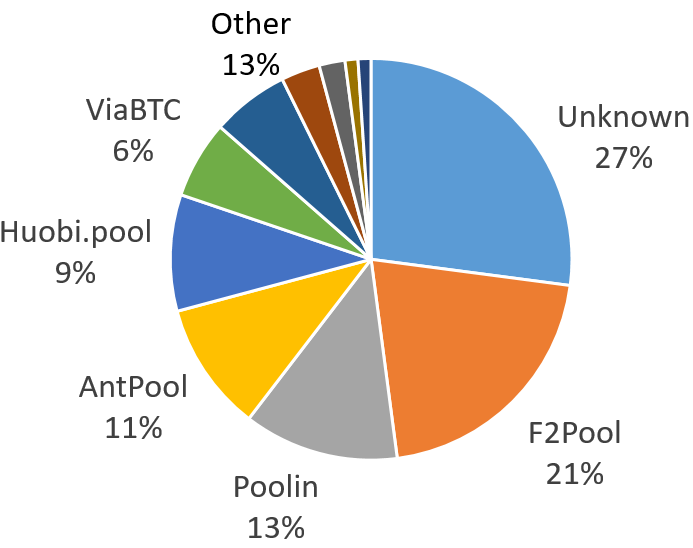
\includegraphics[scale=0.5]{media/hashrate-distribution.PNG}
\end{figure}

While a \textit{sufficiently} distributed network may mean that the computational power of an entity should never exceed 50\% or more of the global hash rate, a higher degree of fragmentation would be preferred for a truly secure network.

\section{Harberger Tax}
\label{section:harberger-tax}

The Harberger Tax \cite{posnerweyl2017} is an economic policy that aims to prevent unequal distribution of property through two rules:

\begin{itemize}
  \item Owners assign a self-assessed value to their property and pay a proportional tax.
  \item The owner is unable to prevent anybody from purchasing their property at their previously set price.
\end{itemize}

The purpose of the first rule is to discourage owners from monopolising their property by assigning a prohibitively high price to prevent others from purchasing as they themselves would have to shoulder the proportional tax. The next rule ensures the mobility of property and that there is no incentive to invest in their property as it is likely to be taken at any given point. This combats the issue of price inflation where an owner may ``hold" their property and increase demand and inflate the price. It will also ensure owners do not set their price too low to avoid taxation.

\section{Strategic Game}
\label{section:strategic-game}

A model can be considered a strategic game if it consists of a finite set of decision-makers $N$ from which each decision-maker has a non-empty set of action profiles $A_i$ that are non-revocable and will be executed simultaneously based on associated preferences \cite[Section 2.1]{osborne1994}. A key factor is that each decision-maker's preferences must also take into account all possible decisions in the game. This definition can be applied to a wide variety of scenarios including the economic model in this proposal, with participants acting as the decision-makers, and their actions being based on not only their own circumstances, but also the actions of other participants.

Once players and their strategies are defined, a table can be constructed in the following format:

\begin{table}[H]
  \centering
  \caption{Example of a finite game with two players}
  \label{table:nashexample}
  \begin{tabular}{|l||*{5}{c|}}\hline
    \backslashbox{Player A}{Player B} & \makebox{Strategy 1} & \makebox{Strategy 2} \\
    \hline \hline
    Strategy 1                        & $a_1$, $b_1$         & $a_1$, $b_2$         \\ \hline
    Strategy 2                        & $a_2$, $b_1$         & $a_2$, $b_2$         \\ \hline
  \end{tabular}
\end{table}

From \cref{table:nashexample}, each cell represents a game in which Player A and Player B each chose a particular strategy which results in a \textit{payoff function} that represents the outcome of the game if the decisions in that cell were taken.

\subsection{Nash Equilibrium} \label{section:nash}

Given a strategic game as defined in \cref{section:strategic-game}, the Nash equilibrium is the proposed \textit{steady state} in which all players are acting based on the \textit{best decision} they can while aware of the actions their opponent(s) will take \cite[Section 2.2]{osborne1994}. Once the strategies of all players, the possible decisions, and all possible game states are defined (at least in natural language) according to the requirements of a strategic game, a Nash equilibrium exists for any action profile in which all players make a decision such that no player can make a decision that results in an outcome more preferred than the current game state. Determining the Nash equilibrium may yield strategies to ensure participants are not incentivised to deviate from the expected behaviour and gain an unfair advantage. 

\subsection{Auctions} \label{section:auctions}

An auction can be considered a strategic game with players, each with a set of strategies and corresponding payoffs for strategy combinations. There are multiple types of auctions \cite{auctions1987} but the most common are:

\begin{itemize}
    \item First price sealed bid auction - Bidders each make a single private bid simultaneously. The highest bidder wins and pays the amount bid.
    \item Second price sealed bid auction - Similar to first price sealed bid, however the highest bidder pays the second highest amount bid.
    \item Open ascending auction - Bidders make increasingly higher bids, until no bidder is willing to pay more.
    \item Open descending bid auction - The price is set excessively high and gradually lowered until a bidder is willing to pay the amount.
\end{itemize}

The bidders themselves are generally modelled with the following factors in mind that may be relaxed to introduce variation in the auction:

\begin{itemize}
    \item Risk-adversity - Bidders would be more or less likely to bid higher on an item given how risk-averse they are.
    \item Information - All bidders should have equal access to information.
    \item Valuation - Each bidder holds the item at a different value individually based on a probability distribution.
    \item Payment - No incentives or royalties are factors in the valuation of the item.
\end{itemize}

\section{Markov Chains}

Markov chains are used to model stochastic systems through a set of states and transitions in either a discrete or continuous time state space. To be eligible for modelling with a Markov chain, a system must be predictable no matter it's current state (i.e. memoryless) \cite{karlin2012first}. In other words, each outgoing transition $t$ from a state $X_n$ has an associated probability that must be based purely on the information present in the state. The probability distributions given by the transitions may then be used to determine the reachability of a state $X_n$ through a set of transitions (or path) $S_t = \{t_0, t_1, \ldots, t_n\}$ with $P(X_n) = \prod_{i=0}^n P(t_i)$.

\section{Related Work}

Two Phase PoW \cite{bastiaan2015} introduces an additional puzzle that requires the use of a private key to sign the work done. While this method would discourage outsourcing, it essentially negates any possibility of public pools that miners rely on for reduced variance. 

P2Pool \cite{p2pool} is an attempt at creating a completely decentralised mining pool (i.e. without a supervisor) but it is riddled with technical issues, high overhead, and much higher variance compared to other pools. 

Smartpool \cite{smartpool2017} is another proposed solution in which the pool is orchestrated via a smart contract (a self-executing ) on the Ethereum blockchain. This is a valid solution that may solve the centralisation of authority for public pools, however there is no incentive for private pools to utilise such a method. 

NiceHash and many other similar platforms, are cryptocurrency hash power brokers in which members can rent hashing power to contribute to a pool of their choice. They make no attempts to address the issue of authority centralisation, rather, their platform enables and encourages it.


\chapter{Formal Definition}

\section{System Overview}

The game requires the following entities:

\begin{itemize}
    \item Any number of \textit{miners} who contribute computational power.
    \item The \textit{pool} that manages and allocates the dedicated computational power into \textit{chunks}.
    \item The \textit{orchestrator} that delegates work to participants, holds unowned chunks.
    \item Any number of \textit{participants} (who may be miners) who purchase and sell the authority over the computational power through ownership of chunks.
\end{itemize}
    
For the purposes of this project, the orchestrator and pool act as a single entity (though an implementation could be based on any number of means such as a dedicated server or smart contract). The ownership of each chunk is taxed according to the Harberger tax (refer to \cref{section:harberger-tax}), with some additions: 

\begin{itemize}
    \item When a participant wishes to purchase a chunk, an auction is initiated. During which, any other participant may chose to participate and bid for the chunk.
    \item When a participant is unable to afford the tax, they relinquish ownership of their chunk. 
    \item Any unowned property is returned to a global pool of unowned property that participants may attempt to purchase through auction starting at the pools sale price.
\end{itemize}

Between each block validated, the orchestrator initiates the trade phase. During this phase, participants may initiate auctions and compete for the ownership of chunks. At the end of the trade phase, participants are taxed according to the number of chunks in their possession and their self-assessed valuation. This trade phase may occur multiple times between validated blocks or once per any number of validated blocks depending on the orchestrator. In the event the pool successfully validates a block, the reward is distributed according to the number of chunks in a participants possession.

\section{Parameterisation} \label{section:parameterisation}

The economic model can be broken down into the following components to create an approximated strategic game.

\subsection{Chunks}

All computational power dedicated to the system will be divided on the basis of a predefined number of chunks to form arbitrary discrete units of computational power. While it is unknown whether or not computational power can be divided based on an arbitrary number for a practical implementation, the computational power represented by each chunk will be equal for the purposes of modelling the system.

\subsection{Participant}

The participants are individuals who may or may not have ownership of some amount of computational power but participate in the system in order to buy and sell chunks of computational power. A participant may be defined as:

\begin{equation}
    \rho := (x, p_s, p_b, f(s))
\end{equation}

\noindent Where the parameters are as follows:
\begin{itemize}
    \item $x$ - Owned chunks - The number of chunks owned by the participant.
    \item $p_s$ - \textbf{P}rice of \textbf{s}ale - The self-evaluated price set by the participant on their owned chunks.
    \item $p_b$ - \textbf{B}uying \textbf{p}rice - The price at which the participant purchased a chunk during an auction.
    \item $f(s)$ - \textbf{F}unction mapping a \textbf{s}tate to the participants decision.
\end{itemize}

During each interval, the participant may chose to initiate an auction given their balance is sufficient or to withhold and not take any action (refer to \crefrange{equation:participantactions}{equation:participantactionsend} for more details).

\subsection{Pool}

The pool acts as the conceptual host of the system, orchestrating auctions and rewarding participants relative to the block time. It is also responsible for managing the tax, dividing, and allocating chunks. A functional implementation would ideally be decentralised and deployed on a blockchain. A blockchain can be defined as:

\begin{align}
    P :=&\; (C, H, t, r, S_\rho) \\
    S_\rho =&\; \{\rho_0, \rho_1, \ldots, \rho_n\}
\end{align}

\noindent Where the parameters are as follows:
\begin{itemize}
    \item $C$ - total \textbf{c}hunks - The total number of chunks to divide contributed computational power.
    \item $H$ - \textbf{H}ash rate - The total hash-rate the contributed computational power is capable of.
    \item $t$ - \textbf{T}rade intervals - the time interval at which a round of trade is executed relative to the block time.
    \item $r$ - Tax \textbf{r}ate - The amount retained by the pool prior to distributing the reward, proportional to the participants price and number of owned chunks.
    \item $S_\rho$ - \textbf{S}et of participants - The participants contributing to this pool.
\end{itemize}

\subsection{blockchain}

An imitation of a real-world blockchain. For the purposes of the model, the actual creation and validation of the block is considered a constant. The discount factor may be used to imitate the depreciation in value of the cryptocurrency. Each blockchain can be defined as:

\begin{align}
    B :=&\; (\mathbb{R}, \mathbb{H}, b, d, S_{po}) \\
    S_{po} =&\; \{P_0, P_1, \ldots, P_n\}
\end{align}

\noindent Where the parameters are as follows:
\begin{itemize}
    \item $\mathbb{R}$ - Block \textbf{r}eward - The value awarded on successfully validating a block of an arbitrary unit.
    \item $\mathbb{H}$ - Global \textbf{h}ash rate - The total computational power dedicated to the blockchain.
    \item $b$ - \textbf{B}lock time - The interval on which a new block is created.
    \item $d$ - \textbf{d}iscount factor - The rate at which the valuation of the blockchains currency depreciates over time.
    \item $S_{po}$ - \textbf{S}et of \textbf{po}ols - The Pools contributing computational power to this blockchain.
\end{itemize}

\subsection{Game}

Containing all the components defined above, the game $G$ is defined to be:

\begin{align}
    G :=&\; (T_i, S_b) \\
    S_b =&\; \{B_0, B_1, \ldots, B_n\}
\end{align}

\noindent Where the parameters are as follows:
\begin{itemize}
    \item $T_i$ - \textbf{T}ime \textbf{i}nterval - Represents a discrete time interval $i \in [0 \rightarrow \infty)$, that dictates a change in the state at each observed increment
    \item $S_b$ - \textbf{S}et of \textbf{B}lockchains - the blockchains that exist in the Universe of Discourse.
\end{itemize}

\section{Relations}

\noindent Expected reward for the ownership of a chunk
\begin{equation} \label{equation:chunkreward}
    R = \frac{\mathbb{R}}{c} \times \frac{H}{\mathbb{H}}
\end{equation}

\noindent Reward per chunk with taxation and discount factor applied
\begin{equation} \label{equation:rewarddiscounted}
    R(d) = R \times \left( 1 - r \right) \times \left( \frac{1}{1 + d} \right)^{d}
\end{equation}

\noindent Amount taxable
\begin{equation} \label{equation:tax}
    t(x) = x \times p_s \times (1 - r)
\end{equation}

\noindent Instantaneous profit from a purchase
\begin{equation} \label{equation:profitpurchase}
    p_{purchase} = (x + y) \times R - t(x) - t(y) - y \times p_b
\end{equation}

\noindent Instantaneous profit from withholding
\begin{equation} \label{equation:profitheld}
    p_{held} = x \times R - t(x)
\end{equation}

\noindent Instantaneous profit from a sale
\begin{equation} \label{equation:profitsale}
    p_{sale} = (y \times p_s)
\end{equation}

At time $T_0$, all participants begin with $x = 0$ and a randomised amount of funds. Between each interval $T_i$ to $T_{i + 1}$, participants will have an opportunity to initiate an auction for any of the available chunks from the pool at a starting rate of $p_p$ or from any of the other participants at their set price $p_s$ while keeping in mind their potential profit from \crefrange{equation:profitpurchase}{equation:profitheld}. A reward is distributed to chunk owners according to \cref{equation:chunkreward} or \cref{equation:rewarddiscounted} depending on the discount factor. Finally, a tax is deducted from each participant according to \cref{equation:tax} where $x = participant.x$ at $T_{i + 1}$.


\input{ch3/state-diagrams}


\chapter{Design and Implementation}

\section{PRISM Games}

PRISM is a probabilistic model checker that enables automatic verification of systems with stochastic behaviour and provides a property checker for verifying specific properties \cite{prism}. PRISM-games is an extension to prism that adds support for turn based or concurrent multi-player games \cite{prismgames}. 

Abstracting the auction to a constant in the proposed model, the game may be modelled in a discrete time Markov chain using trade intervals and block time as signals for transitions. Furthermore, applying a discount factor and threshold ensures the number of states can be reduced to a finite set. In doing so, the game can then be modelled in PRISM-games in an attempt to verify the presence of a Nash equilibrium. 


\section{Deterministic State Generator}

As PRISM-games was insufficient (refer to \cref{section:prism-results} ) for verifying the equality of the game, a custom modeller was created in an attempt to verify the game through a different technique. The deterministic state generator mimics the functionality of PRISM-games, generating the set of all possible states and transitions. In addition, querying paths and reachability can be tailored to the custom implementation rather than conform to PRISM-games property syntax.

\subsection{Parameterisation}

The state generator accepts the following as parameters as a basis to creating states:

\begin{itemize}
    \item $r$ - Tax rate.
    \item $d$ - Discount factor.
    \item $R$ - Expected reward per owned chunk.
    \item $t$ - Threshold at which to consider the reward as too low.
\end{itemize}

For the purposes of modelling, each participant is represented by an object with the following properties:

\begin{itemize}
    \item $balance$ - the current value in the participants possession as a unit of the block reward.
    \item $chunks$ - the current number of chunks in the participants possession.
    \item $chance$ - A chance used to determine if a participant will participate, initiate an auction, or withhold.
\end{itemize}

Each state created in the state generator can be defined as:

\begin{align}
    S :=&\; (c, d, a, P) \\
    P =&\; \{p_0, p_1, \ldots, p_n\}
\end{align}

\noindent Where the parameters are as follows
\begin{itemize}
    \item $c$ - The probability of reaching this state. Refer to \cref{equation:stateprobability} below.
    \item $d$ - The number of steps to reach this state (or depth).
    \item $a$ - The action taken to transition to this state.
    \item $P$ - A set of participant objects containing their initial state.
\end{itemize}

Each state represents the funds and chunks of each participant and maintains a reference to future states. Algorithm \ref{algorithm:generatestates} details the recursive process of generating states.

An action represents the decision made by one or many participants to change the current state or by the distribution of a reward. It may be represented as:

\begin{align}
    A :=&\; (\tau, c, S_t) \\
    S_t =&\; {t_0, t_1, \ldots, t_n} \\
    \tau \in&\; \{\textsc{Reward, Purchase}\}
\end{align}

\noindent Where the parameters are as follows
\begin{itemize}
    \item $\tau$ - The transition type.
    \item $c$ - The probability of this transition occurring. Refer to \crefrange{equation:participantactions}{equation:participantactionsend} below.
    \item $S_t$ - The set of transactions executed in this transition. Zero or more discrete transactions such that $\forall t \in S_t : \nexists \; t' \in S_t : t.buyer = t'.buyer$.
\end{itemize}

A transaction contains details about the transferal of chunk ownership between participants and can be defined as the following:

\begin{equation}
    T := (b, s, p)
\end{equation}

\noindent Where the parameters are as follows
\begin{itemize}
    \item $b$ - The buyer who initiated the transaction.
    \item $s$ - The seller from which the chunk will be transferred from.
    \item $p$ - The price at which the buyer is purchasing for.
\end{itemize}

\subsection{Modelling}

In order to facilitate the modelling of the game as a Markov chain, the probability of a participants actions can be defined on set of participants $P$ and the above parameters:

\begin{align} \label{equation:participantactions}
    \forall b \in Buyers &: b.chance > 0 \land b.funds \geq 1 \\
    \forall s \in Sellers &: b.chunks \geq 1 \\
    P(b_{purchase}) &= \frac{b.chance}{Sellers.length} \label{equation:probabilitypurchase}\\
    f(s) &= \label{equation:participantactionsend}
        \begin{cases}
            P(b_{purchase})     & \text{if $b$ chooses to purchase} \\
            P(1 - b_{purchase}) & \text{else if $b$ can purchase but chooses to withhold} \\
            1                   & \text{else if $b$ has insufficient funds to purchase}
        \end{cases}
\end{align}

The probability of reaching a state $X$ may then be calculated as the product of actions taken to reach it:

\begin{equation}
    P(X) = P(X_{prev}) \times \prod_{i=1}^{Buyers} action(b_i) \label{equation:stateprobability}
\end{equation}

The expected reward may then be calculated using the product of the balances at each end state and the state probability. Given a set of end states $\{X_{x \mid 0}, X_{x \mid 1}, \ldots, X_{x \mid n}\}$, where $X_{x \mid i}$ represents the balance of participant $x$ at the $i$th state $X$. Hence for participant $x$, the expected reward can be calculated as:

\begin{equation} \label{algorithm:state-expected-reward}
    \mathbb{E}(R(x \mid i)) = \sum_{i = 0}^n X_{x \mid i} \times P(X_{x \mid i})
\end{equation}

\subsection{Algorithms}

The following algorithms should be the minimum required logic in order to create a Deterministic State Generator according to the above game specifications detailed in previous sections.

Algorithm \ref{algorithm:generatestates} below shows the process for which states were recursively generated. A new state is created for each potential combination or subset of possible transactions the participants are able to take in the current state until no more actions can be taken or the reward is reduced below a threshold due to the discount factor. It accepts the following parameters:

\begin{itemize}
    \item $S_\rho$ - The set of participants.
    \item $state$ - The new state.
    \item $depth$ - The current depth.
\end{itemize}

\begin{algorithm}[H]
\caption{Recursive state generator}
\label{algorithm:generatestates}
\begin{algorithmic}[1]
\Procedure{generateStates}{$S_\rho, state, depth$}
    \State $r \gets R(depth)$ \Comment{refer to \cref{equation:rewarddiscounted}}
    \If{$r < t$}
        \State \Return
    \EndIf
    \State $state.subStates \gets \textsc{empty set of State}$
    \State $S_t \gets \textsc{generateTransactions}(S_\rho)$ \Comment{refer to \cref{algorithm:generatetransactions}}
    \State $S_c \gets \textsc{calculateStateChance}(state, S_t, S_\rho)$ \Comment{refer to \cref{algorithm:calculatestatechance}}
    \For{$i \in [0, S_t.length)$}
        \State $action \gets new \textsc{ Action}(S_t[i], S_c[i])$
        \State $S_\rho' \gets \textsc{applyAction}(S_\rho, action)$ \Comment{refer to \cref{algorithm:applyaction}}
        \State $subState \gets new \textsc{ State}(S_\rho', action)$
        \State $state.subStates \gets state.subStates \cup \{subState\}$
        \State $\textsc{generateStates}(S_\rho', subState, depth + 1)$
    \EndFor
\EndProcedure
\end{algorithmic}
\end{algorithm}

Algorithm \ref{algorithm:generatetransactions} generates all possible combinations and subsets of transactions given the current participants state. It accepts the set of participants $S_\rho$ as the basis for determining possible transactions.

\begin{algorithm}[H]
\caption{Transaction combination generator}
\label{algorithm:generatetransactions}
\begin{algorithmic}[1]
\Procedure{generateTransactions}{$S_\rho$}
    \State $B \gets \{ b \in S_\rho \mid b.balance \geq 1 \land b.chance > 0 \}$
    \State $S \gets \{ s \in S_\rho \mid s.chunks \geq 1 \}$
    \State $transactionSets \gets \textsc{empty set of set of Transaction}$
    \For{$b \in B$}
        \State $set \gets \textsc{empty set of Transaction}$
        \For{$s \in S$}
            \State $set \gets set \cup \{new \textsc{ Transaction}(b, s)\}$
        \EndFor
        \State $transactionSets \gets transactionSets \cup \{set\}$
    \EndFor
    \State $result \gets \textsc{empty set of set of Transaction}$
    \State $unvisited \gets TransactionSets$
    \While{$unvisited \neq \emptyset$}
        \State $set \gets unvisited.\textsc{pop}()$
        \For{$transaction \in set$}
            \For{$otherSet \in unvisited$}
                \For{$otherTransaction \in otherSet$}
                    \If{$transaction.seller \neq otherTransaction.seller$
                        \State $\lor \; transaction.seller.chunks > 1$}
                        \State $result \gets result \cup \{[transaction, otherTransaction]\}$
                    \EndIf
                \EndFor
            \EndFor
            \State $result \gets result \cup \{[transaction]\}$
        \EndFor
    \EndWhile
    \State \Return $result$
\EndProcedure
\end{algorithmic}
\end{algorithm}

Algorithm \ref{algorithm:calculatestatechance} below determines the probability distribution of states belonging to a parent state. It considers all participants with the ability to purchase and determines the probability of each action occurring. Participants who are not in the set $B$ defined in line 2 are considered to not be eligible for purchasing and are not considered as they would not have a choice. The algorithm accepts the following parameters: 

\begin{itemize}
    \item $T$ - The set of transitional transactions.
    \item $S_\rho$ - The set of participants.
\end{itemize}

\begin{algorithm}[H]
\caption{Determines the chance of a state given a transition and parent state. }
\label{algorithm:calculatestatechance}
\begin{algorithmic}[1]
\Procedure{calculateStateChance}{$T, S_\rho$} 
    \State $B \gets \{ b \in S_\rho \mid b.balance \geq 1 \land b.chance > 0 \}$
    \State $S \gets \{ s \in S_\rho \mid s.chunks \geq 1 \}$
    \State $chances \gets 1$
    \For{$b \in B$}
        \If{$t \in T : t.buyer = b$}
            \State $chances \gets chances \times \frac{b.chance}{length(S - b)}$
        \Else
            \State $chances \gets chances \times (1 - b.chance)$
        \EndIf
    \EndFor
    \State $total \gets 1$
    \State \Return $chances$
\EndProcedure
\end{algorithmic}
\end{algorithm}

Algorithm \ref{algorithm:applyaction} below updates the state of each participant to apply a transition to the state owning the given set of participants. It accepts the following parameters:

\begin{itemize}
    \item $S_\rho$ - The set of participants.
    \item $a$ - The transitional action to apply to the state
\end{itemize}

\begin{algorithm}[H]
\caption{Applies a transition on a state}
\label{algorithm:applyaction}
\begin{algorithmic}[1]
\Procedure{applyAction}{$S_\rho, a$}
    \Switch{$a.\tau$}
        \Case \textsc{Reward}
            \For{$\rho \in S_\rho$}
                \State $\rho.funds \gets \rho.funds + R(\rho.chunks)$ \Comment{refer to \cref{equation:rewarddiscounted}}
            \EndFor
        \EndCase
        \Case \textsc{Purchase}
            \For{$t \in action.S_t$}
                \State $t.buyer.funds \gets t.buyer.funds - t.price$
                \State $t.buyer.chunks \gets t.buyer.chunks + 1$
                \State $t.seller.funds \gets t.seller.funds + t.price$
                \State $t.seller.chunks \gets t.seller.chunks - 1$
            \EndFor
        \EndCase
    \EndSwitch
\EndProcedure
\end{algorithmic}
\end{algorithm}

\subsection{Implementation}

The source code for the implementation used for the purposes of this project can be found on Gitlab \footnote{\url{https://gitlab.com/harberger-tax/state-diagram-generator}}. Created in TypeScript \cite{typescript2020}, it provides a command line interface with a number of options to programmatically change how the resultant states are generated. 

The program was created in TypeScript due to familiarity and syntactical convenience, with fast prototyping and compilation, it was preferable for fast prototyping. In addition to the generator, a visualisation utility was added utilising Mermaid \cite{mermaid} which enabled rendering smaller scale state diagrams for visual inspection. Additionally, as it is natively supported in all browsers, it is trivial to embed functionality into other projects such as the demonstration (refer to \cref{section:demonstration}). With the system used for experimentation in \cref{appendix:computerspecs}, a maximum depth of 30 yielded over 2.5 million states in ~40 seconds and utilising over 5GB of ram. At a discount factor of 0.01, a tax rate of 0.05, and a threshold of 0.009, the maximum depth required at 4713 would not be feasible as the amount of memory required to create the complete set states far exceed the computational resources available.

Figure \ref{figure:state-diagram-small} below shows a small sample set of states generated with participants having a chance of 0.9 and a maximum depth of 1. Each node contains information on the current state of each participant in the form P$i$: $c$, $f$ where $i$ is the ID of the participant, $c$ is the owned chunks, and $f$ is the current balance. Each arrow represents a transition in which either the distribution of chunks or funds of any participant observes a change and are labelled with the chance for the transition to occur and the reason for the transition (A purchase, reward, or no change occurred).

\begin{figure}[H]
  \centering
  \caption{Deterministic state generator minimal example}
  \label{figure:state-diagram-small}
  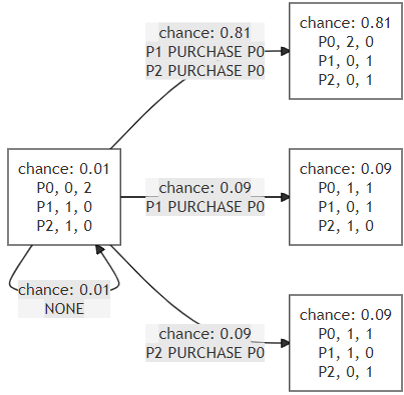
\includegraphics[width=0.5\textwidth]{media/state-diagram-small.PNG}
\end{figure}


\section{Simulation}

\subsection{Parameterisation}

The simulation makes use of all variables defined in \cref{section:parameterisation} above and aims to be as close a representation of a potential game run as possible. Unlike the Deterministic State Generator, the simulation maintains a single persistent state that is updated based on a semi-random process rather than generating possible states.

\subsection{Modelling}

In order to facilitate increased complexity in a participants decision-making process, the participant can be represented as the following:

\begin{align}
    P &= (funds, chunks, chance, wantedChunks, \sigma) \\
    \sigma &\subseteq \{\textsc{First, SkipFirst, Alternate, Chance, WantedChunks}\}
\end{align}

\begin{itemize}
    \item $funds$ - The current balance of the participant.
    \item $chunks$ - The chunks currently owned by the participant.
    \item $chance$ - The chance of participating (required if $\textsc{Chance} \in \sigma$).
    \item $wantedChunks$ - The target number of chunks the participant wishes to posess (required if $\textsc{WantedChunks} \in \sigma$).
    \item $\sigma$ - The strategy used to determine participation, can be any individual strategy or a combination of strategies. Each element in $\sigma$ affects the participants predisposition to participate in and initiate auctions.
    \begin{itemize}
        \item \textsc{First} - Guarantee participation in the inital round.
        \item \textsc{SkipFirst} - Guarantee no participation in the initial round.
        \item \textsc{Alternate} - Alternate participation each round.
        \item \textsc{Chance} - Base participation on a randomly generated number against the $chance$ value.
        \item \textsc{WantedChunks} - Avoid participating if the owned chunks is equal or greater to the wanted chunks.
    \end{itemize}
\end{itemize}

The pool model is also augmented with the properties of participants to simulate the expected reward a pool operator might expect from acting as a host for the game. In other words $P_\rho := P \cup p$.

\subsection{Algorithms}

Algorithm \ref{algorithm:simulate} below shows the looped execution of the simulation. The simulation iterates until the reward is reduced below a threshold. At each iteration, if the round matches up to the block interval, a reward may be distributed depending on a random number generated against the pool's global compute share. It accepts the following parameters:

\begin{itemize}
    \item $G$ - The game instance.
    \item $B$ - The blockchain instance.
    \item $P$ - The pool instance.
    \item $S_\rho$ - The set of participants.
\end{itemize}

\begin{algorithm}[H]
  \caption{Simulation event loop}
  \label{algorithm:simulate}
  \begin{algorithmic}[1]
    \Procedure{simulate}{$G, B, P_\rho, S_\rho$}
        \State $round \gets 0$
        \While{$R(round) > t$}
            \If{$round \mod \left( \left\lfloor \frac{B.b}{P_\rho.t} \right\rfloor \right) \equiv 0$}
                \State $\textsc{reward}(S_\rho, B, P_\rho)$ \Comment{refer to \cref{algorithm:reward}}
            \EndIf
            \State $bidders \gets \{ b \in S_\rho \mid b.balance \geq 1 \}$
            \For{$p \in \{ p \in S_\rho \mid p.chunks \geq 1\}$}
                \State $\textsc{auction}(bidders, p)$ \Comment{refer to \cref{algorithm:auction}}
            \EndFor
            \State $round \gets round + 1$
        \EndWhile
    \EndProcedure
  \end{algorithmic}
\end{algorithm}

Algorithm \ref{algorithm:reward} below rolls a generates a random float in the interval $[0, 1]$ against the pool's global compute share. If the roll was successful, the reward is distributed amongst the participants, with the leftover awarded to the pool. It accepts the parameters:

\begin{itemize}
    \item $S_\rho$ - The set of participants.
    \item $B$ - The blockchain instance.
    \item $P_\rho$ - The pool instance.
\end{itemize}

\begin{algorithm}[H]
\caption{Reward system for pool participants}
\label{algorithm:reward}
\begin{algorithmic}[1]
\Procedure{reward}{$S_\rho, B, P_\rho$}
    \State $roll \gets \textsc{randomFloat(0, 1)}$ \Comment{a random decimal in the range $[0, 1]$}
    \If{$roll > \frac{P_\rho.H}{B.\mathbb{H}}$} 
        \State \Return \Comment{Pool did not validate the block} 
    \EndIf
    \State{$leftover \gets r$}
    \For{$\rho \in S_\rho$}
        \State $amount \gets R(\rho.chunks)$ \Comment{refer to \cref{equation:rewarddiscounted}}
        \State{$\rho.funds \gets \rho.funds + amount$}
        \State{$leftover \gets leftover - amount$}
    \EndFor
    \State{$P_\rho.funds \gets P_\rho.funds + leftover$}
\EndProcedure
\end{algorithmic}
\end{algorithm}

Algorithm \ref{algorithm:auction} below simulates the auction process for a standard open auction in which participants bid for the highest price. It accepts the parameters:

\begin{itemize}
    \item $B$ - The current bidders.
    \item $\rho_s$ - The current seller.
    \item $price$ - The current price or last bid.
    \item $\rho_b$ - The last bidder.
\end{itemize}

\begin{algorithm}[H]
\caption{Recursive auction resolution}
\label{algorithm:auction}
\begin{algorithmic}[1]
\Procedure{auction}{$B$, $\rho_s$, $price$, $\rho_b$}
    \If{$B = \emptyset$}
        \State{$\rho_b.funds \gets \rho_b.funds - price$}
        \State{$\rho_b.ownedChunks \gets \rho_b.ownedChunks + 1$}
        \State{$\rho_s.funds \gets \rho_s.funds + price$}
        \State{$\rho_s.ownedChunks \gets \rho_s.ownedChunks - 1$}
        \State \Return
    \EndIf
    \State{$bidder_{max} \gets \rho_b$}
    \State{$bid_{max} \gets price$}
    \For{$bidder \in B$}
        \State{$bid \gets bidder.\textsc{bid}(price)$}
        \If{$bid > bid_{max}$}
            \State{$bid_{max} \gets bid$}
            \State{$bidder_{max} \gets bidder$}
        \EndIf
    \EndFor
    \State{$B' \gets \emptyset$}
    \For{$bidder \in B$}
        \State $p \gets \textsc{checkParticipation}(bidder, \rho_s, bid_{max}, bidder_{max})$ \Comment{refer to \cref{algorithm:checkparticipation}}
        \If{$p = true$}
            \State{$B' \gets B' \cup bidder$}
        \EndIf
    \EndFor
    \State{\Return $\textsc{auction}(B', \rho_s, bid_{max}, bidder_{max})$}
\EndProcedure
\end{algorithmic}
\end{algorithm}

Algorithm \ref{algorithm:checkparticipation} below considers the participants current state, the current bid, and the participants strategy in order to determine if the participant should (or can) participate. The parameters are:

\begin{itemize}
    \item $\rho$ - The participant.
    \item $\rho_s$ - The current seller.
    \item $price$ - The current bid.
    \item $\rho_b$ - The current highest bidder.
    \item $round$ - The current round.
\end{itemize}

\begin{algorithm}[H]
\caption{Participant decision making process}
\label{algorithm:checkparticipation}
\begin{algorithmic}[1]
\Procedure{checkParticipation}{$B, \rho_s, price, \rho_b, round$}
    \If{$\rho = \rho_s \lor \rho = \rho_b \lor price > \rho.funds$
            \State $\lor \;(\textsc{WantedChunks} \in \rho.\sigma$
            \State $\land \; \rho.ownedChunks \geq \rho.wantedChunks)$
            \State $\lor \; (\textsc{SkipFirst} \in \rho.\sigma$
            \State $\land \; round = 0)$
    }
        \State \Return false
    \EndIf
    \If{$\textsc{First} \in \rho.\sigma \land round = 0$}
        \State \Return true
    \EndIf
    \If{$\textsc{Alternate} \in \rho.\sigma$}
        \If{$(\textsc{First} \in \rho.\sigma \land round \pmod 2 = 0)$
                \State $\lor \; (\textsc{SkipFirst} \in \rho.\sigma \land round \pmod 2 \neq 0)$
        }
            \State \Return true
        \EndIf
    \EndIf
    \If{$\textsc{Chance} \in \rho.\sigma \land \textsc{randomFloat}(0, 1) < \rho.chance$}
        \State \Return true
    \EndIf
    \State \Return false
\EndProcedure
\end{algorithmic}
\end{algorithm}

\subsection{Implementation}

The source code for the implementation used for the purposes of this project can be found on Gitlab \footnote{\url{https://gitlab.com/harberger-tax/simulation}}. With similar reasoning to the deterministic state generator, the simulation is written in Typescript with the addition of Chart.js \cite{chartjs} to visualise data. 


\chapter{Results}

% \todo[inline]{
%     how you collected and analysed your data – you only need to include enough detail that another expert in the field could repeat what you've done (you don't have to detail field standard techniques or tests) \\
%         - simulation \\
%         - prism model \\
%         - state diagram generator \\
%     why you chose to collect specific data \\
%     how this data will help you to answer your research questions \\
%     why you chose the approach you went with. \\
% }

% \todo[inline]{
%     specify the data you collected and how it was were prepared for analysis \\
%     describe the data analysis (e.g. define the type of statistical test that was applied to the data) \\
%     describe the outcome of the analysis \\
%     present a summary and descriptive statistics in a table or graph.
% }

All experimentation was done on the system detailed in \cref{appendix:computerspecs} using the implementations defined in the previous sections. The repository containing all source code is at \url{https://gitlab.com/harberger-tax} and is freely accessible should it be of use to anyone.

\section{PRISM-games} \label{section:prism-results}

\subsection{Implementation}

The implemented model can be found in \cref{appendix:prism-model} or on Gitlab \footnote{https://gitlab.com/harberger-tax/prism-models}. It is written as a concurrent stochastic game (\texttt{csg}) with three players (a pool and two participants) and requires the following parameters: 

\begin{itemize}
    \item $p$ - The probability of player 1 purchasing.
    \item $q$ - The probability of player 2 purchasing.
    \item $tr$ - The tax rate.
    \item $dr$ - The discount rate.
\end{itemize}.

The model is split into two phases per round. First, in the decision phase, all participants make a decision on whether or not to participate and if participating, who to purchase from. Next, in the purchase phase, all purchases are executed. The model was split into two phases in order to prevent double-purchasing where both participant may attempt to purchase from a participant with a single chunk.

In order for PRISM-games to verify the model, rewards were associated with each phase. First, an amortised block reward reduced by tax and discount factor is awarded during the decision phase. Next, a participant is rewarded or penalised during the purchase phase if they bought or sold a chunk.

\subsection{Results}

Attempting to build the PRISM-games model more than 120 steps resulted in an unknown error, most likely due to being unable to acquire the necessary memory required, or being unable to support the required number of states. Additionally, there was no easy way to programmatically test with different parameters. Hence, PRISM-games was discarded in favour of a custom implementation with the deterministic state generator.


\section{Deterministic State Generator}

\subsection{Methodology}

As the hardware limitations prevent the creation of complete system models, a smaller subset was utilised for analysis. All systems were created with the following parameters (parameters were inflated to accelerate the decay of reward valuation):

\begin{itemize}
    \item Blockchain 
    \begin{itemize}
        \item Block reward - 1
    \end{itemize}  
    \item Pool 
    \begin{itemize}
        \item Initial chunks - 2
    \end{itemize}
    \item Participants
    \begin{itemize}
        \item Initial funds - 1
        \item Initial chunks - 0
    \end{itemize}
    \item Reward minimum threshold - 0.009
    \item Maximum depth - 15
\end{itemize}

The following metrics were recorded regarding each participants potential expected reward based on different participation chances.

\begin{itemize}
    \item The most equal state (smallest difference in balance).
    \item The least equal state (greatest difference in balance).
    \item Total end states.
    \item Total end states within the given wealth-difference.
    \item Metrics for each participant which includes:
    \begin{itemize}
        \item The number of states reachable with the highest balance.
        \item The highest balance possible.
        \item The number of states reachable with the lowest balance.
        \item The lowest balance possible.
        \item The total number of states within the given wealth-difference.
    \end{itemize}
\end{itemize}

\subsection{Results}

Even before generating any states, some intuitive assumptions can be made regarding the potential outcomes of a game in which only two participants exist:

\begin{itemize}
    \item If both participants purchase from the pool in the first step and continue to purchase from each other or do not purchase at all in consequent steps, they will always be in  equilibrium (i.e. equal balance).
    \item The highest possible balance achievable while in equilibrium is if both participants hold a chunk each and do not purchase.
    \item The results will be symmetric for participants (unless probability or initial state is different).
\end{itemize}

Consider a game in which the initial state is as follows.

\begin{itemize}
    \item Pool - chunks: 2, balance: 0
    \item Participant 1 - chunks: 0, balance: 1
    \item Participant 2 - chunks: 0, balance: 1
\end{itemize}

The expected payout for all action combinations can be seen in \cref{table:payout1} below. 

\begin{table}[H]
  \centering
  \caption{Expected payout for a basic two-player game}
  \label{table:payout1}
  \begin{tabular}{|l||*{5}{c|}}\hline
    \backslashbox{Participant 1}{Participant 2} & \makebox{Skip} & \makebox{Purchase} \\
    \hline \hline
    Skip                                        & 0, 0           & 0, 1 \\ \hline
    Purchase                                    & 1, 0           & 2, 2 \\ \hline
  \end{tabular}
\end{table}

In the case where both participants skip (Skip, Skip), they receive no rewards (having no chunks). If both participants purchase at the same time (Purchase, Purchase), they expend their balance in order to buy the chunk from their opponent and receive an equal amount of funds for selling their chunk to their opponent, resulting in no net change in balance. Then, during the reward phase, both participants receive one unit for having one chunk in their possession. In cases where only one participant purchases (Skip, Purchase), only the purchaser expends their balance but does not receive any as a chunk was not purchased from them. Next, they receive a reward, restoring their balance back to 1. In this case, the participant who opted to skip would consider purchasing a chunk to catch up, returning to the action combination (Purchase, Purchase). Hence, there exists a Nash equilibrium with the action combination (Purchase, Purchase).

A test was run using the generator for participant probabilities ranging from 0.1 to 0.9 for both participants with a tax rate of 0 and 0.2 (the test script can be found in \cref{appendix:testparticipationprobability}). Only one participant is considered as they are symmetrical in all aspects.

\begin{figure}[H]
  \centering
  \caption{Expected reward per combination of participant purchase probability}
  \label{figure:state-expected}
  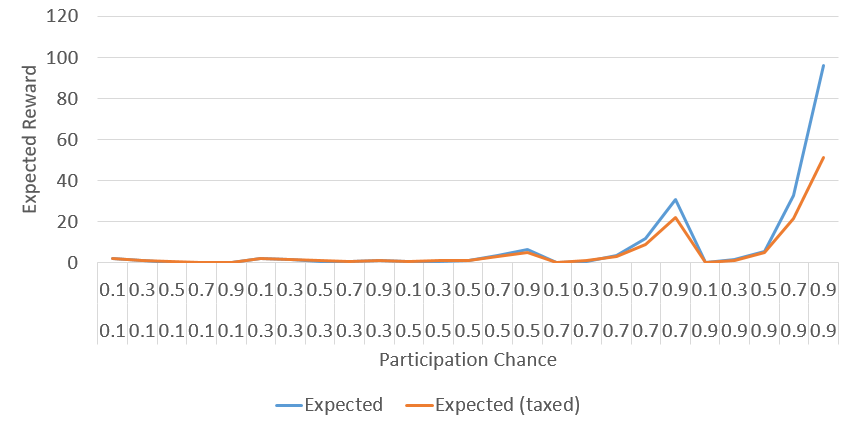
\includegraphics[width=\textwidth]{media/state-expected.PNG}
\end{figure}

The results seen in \cref{figure:state-expected} above shows the expected reward per combination of participation chances. Participant 1 on the bottom row and participant 2 on the top row. It can be observed that higher participation rates yield a higher expected reward, with spikes each time both participation chances reach a relatively high value. This is likely due to the fact that as the product of the probabilities yields the maximum possible chance a state may achieve, reducing the expected reward accordingly. For example, given participants 1 and 2 both have a 0.1 chance to participate, the combination is $0.1 \times 0.1 = 0.01$, meaning the final reward is reduced by x100. Similarly, given participants 1 and 2 both have 0.9 chance to participate, the combination $0.9 \times 0.9 = 0.81$ is significantly higher with at most a 19\% reduction. It is also noted that the impact of the tax becomes more pronounced as the probability to purchase increases. This is likely due to participants being taxed more frequently as they are more likely to possess chunks given the higher purchase probability.

Figure \ref{figure:state-bestworst} below shows the probability of reaching the states with the highest and lowest balance.

\begin{figure}[H]
  \centering
  \caption{Probability of reaching state with highest and lowest balance}
  \label{figure:state-bestworst}
  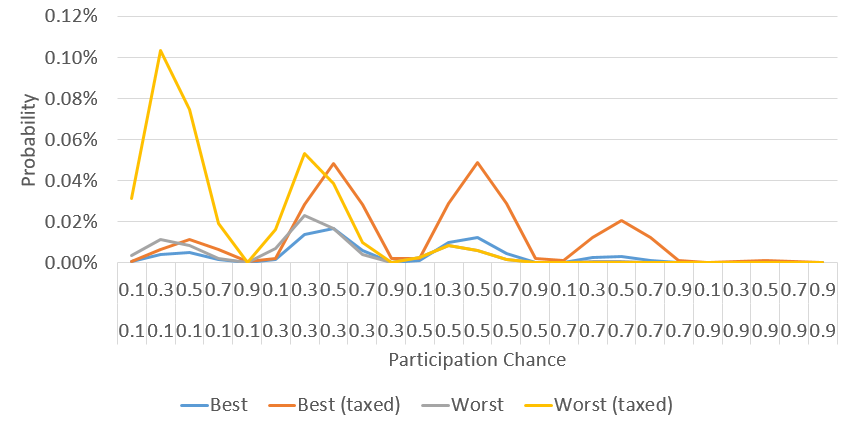
\includegraphics[width=\textwidth]{media/state-bestworst.PNG}
\end{figure}

The peaks in the worst (taxed) trend-line may be due to the low purchase likelihood of the participant directly benefiting the other participant, leading the the largest difference in funds. This was predicted in \cref{table:payout1} in the action combinations (Skip, Purchase). As the purchase probability increases, the peaks reduce in magnitude as probability to reach an equilibrium state increases, decreasing the probability to reach a worst case state. Similarly, the best states are only achievable if neither participant is especially inclined to purchase, increasing the probability of traversing a chain of transitions in which one participant does not purchase chunks, letting the other participant accumulate the rewards unchecked.

Figure \ref{figure:state-expected-tax} below shows the expected reward as tax increases. The test script can be found in \cref{appendix:testparticipationtax} and the raw data can be found in \cref{appendix:state-results-tax} As expected, the reward decreases in a linear fashion as the tax increases.

\begin{figure}[H]
  \centering
  \caption{Expected reward per tax rate}
  \label{figure:state-expected-tax}
  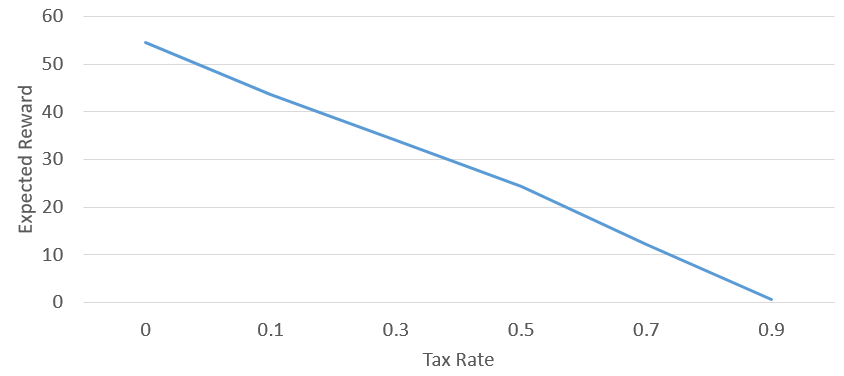
\includegraphics[width=\textwidth]{media/state-expected-tax.PNG}
\end{figure}


\section{Simulation}

\subsection{Methodology}

As the simulation is not limited by hardware, all executions are able to run to completion. All simulations were run with the following parameters (similarly exaggerated to accelerate decay):

\begin{itemize}
    \item Blockchain
    \begin{itemize}
        \item Block reward - 12.5
        \item Global hash rate - 1
        \item Block time - 1
        \item Discount factor - 0.001\%
    \end{itemize}
    \item Pool 
    \begin{itemize}
        \item Hash rate - 0.3 (i.e. 30\%)
        \item Tax rate - 5\%
        \item Trade interval - 0.5
    \end{itemize}
    \item Participants
    \begin{itemize}
        \item Count - 3
        \item Initial chunks - 0
    \end{itemize}
    \item Reward minimum threshold - 0.009
\end{itemize}

\subsection{Results}

Figures \ref{figure:simulation-balance} and \ref{figure:simulation-chunks} are the results of a simulation with three participants, four chunks, and limited to 200 rounds. Figure \ref{figure:simulation-balance} below shows that the general trend is fairly balanced in the beginning but begins to diverge as balances increase. While participant 3 lags behind, this can be explained by the their reduced activity as seen in \cref{figure:simulation-chunks}. Despite this, the average distribution of funds observe a positive trend given the right conditions and do not diverge significantly.

\begin{figure}[H]
  \centering
  \caption{Balance distribution over shortened simulation lifespan}
  \label{figure:simulation-balance}
  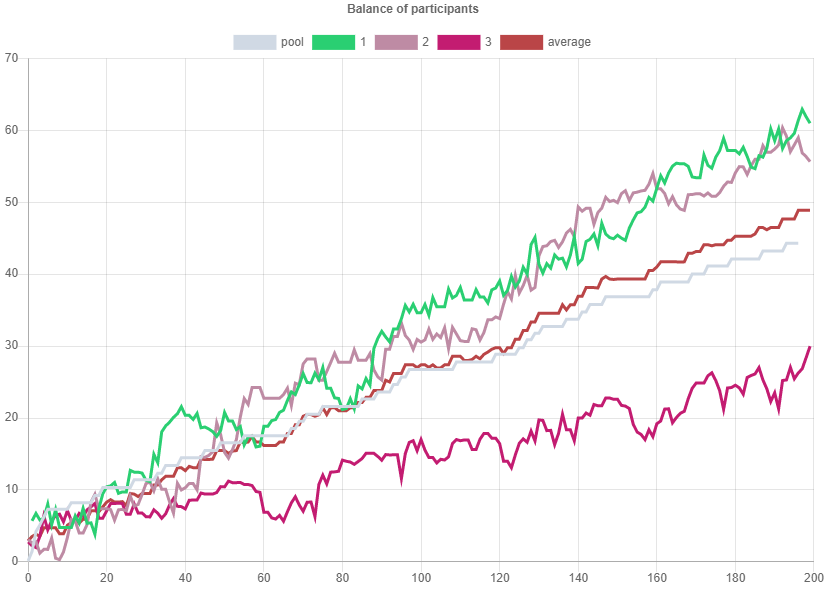
\includegraphics[width=0.8\textwidth]{media/simulation-balance.PNG}
\end{figure}

As seen in \cref{figure:simulation-chunks} below, the transition of funds occurred fairly frequently, effectively reducing any chance a participant may have in holding all the chunks. It is noted that there were several instances when a participant was able to hold all the chunks. while they were never in a participants possession for longer than a single round, it is less than ideal as it is possible for the game to reach such a state. Despite these spikes, the balances did not experience any sudden jumps in correlation to the possession of all chunks. This is likely due to the trade interval being half that of the block time, meaning a participant will likely have to maintain possession of the chunk for two rounds. 

\begin{figure}[H]
  \centering
  \caption{Chunk distribution over shortened simulation lifespan}
  \label{figure:simulation-chunks}
  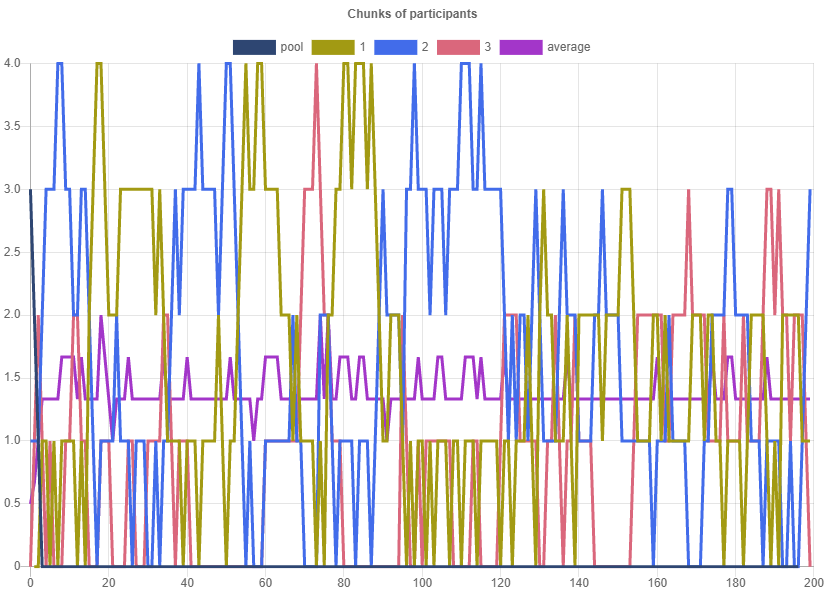
\includegraphics[width=0.8\textwidth]{media/simulation-chunks.PNG}
\end{figure}

Figures \ref{figure:simulation-converge-balance} and \ref{figure:simulation-converge-chunks} are the results of a simulation with three participants, six chunks, and was allowed to run to completion (based on the discount factor and reward threshold). Figure \ref{figure:simulation-converge-balance} shows an ideal situation in which despite varying degrees of growth, the final trend is towards the average. It shows that as participants purchase from one another, they may still have chunks in reserve, accumulating rewards passively as they trade as they are able to consistently maintain ownership of chunks for longer. In this case, the balance is likely to converge despite differing participation probabilities as participants effectively inhibit divergence through consistent trading. It is noted that the number of rounds is less than the previous simulation. This is due to the increased number of chunks resulting in lower rewards per chunk as previously defined by \cref{equation:chunkreward}.

\begin{figure}[H]
  \centering
  \caption{Balance distribution over simulation lifespan with increased chunks}
  \label{figure:simulation-converge-balance}
  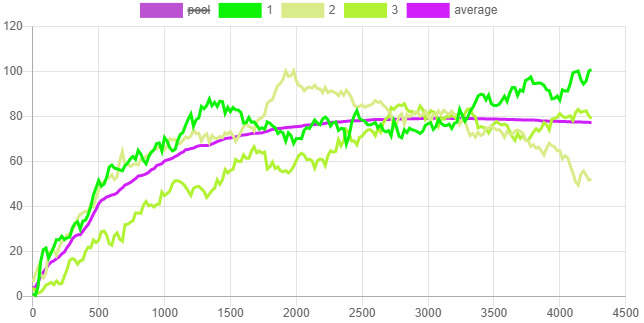
\includegraphics[width=0.8\textwidth]{media/simulation-converge-balance.PNG}
\end{figure}

Figure \ref{figure:simulation-converge-chunks} below shows the maximum difference in chunks held over the lifespan of the simulation. Over the course of the simulation, no participant held more all available chunks for longer than one round, reducing the likelihood of earning the whole balance awarded to the pool.

\begin{figure}[H]
  \centering
  \caption{Averaged chunk distribution over simulation lifespan with increased chunks}
  \label{figure:simulation-converge-chunks}
  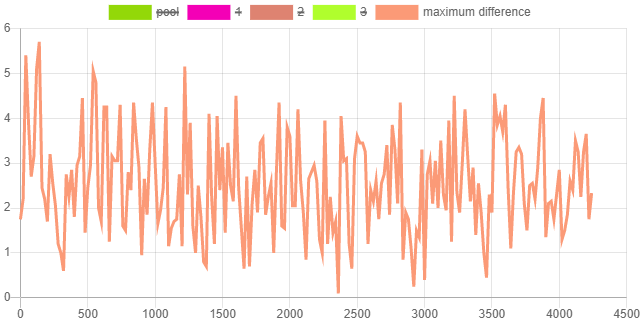
\includegraphics[width=0.8\textwidth]{media/simulation-converge-chunks.PNG}
\end{figure}

Figures \ref{figure:simulation-divergence-balance} and \ref{figure:simulation-divergence-chunks} are the results of a simulation with three participants, two chunks, and was allowed to run to completion (based on the discount factor and reward threshold). As seen in \cref{figure:simulation-divergence-balance} below, the funds appear to diverge as time goes on with one participant reaching close to an no funds. This is likely due to the fact that as the number of chunks is not enough to satisfy all participants, some participants are not able to receive a reward during some rounds and become disadvantaged due to the difference. 

\begin{figure}[H]
  \centering
  \caption{Balance distribution over simulation lifespan with decreased chunks}
  \label{figure:simulation-divergence-balance}
  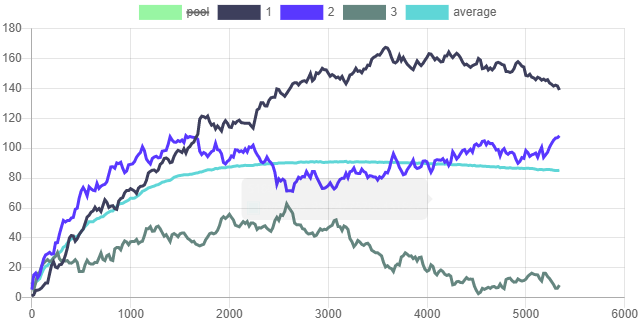
\includegraphics[width=0.8\textwidth]{media/simulation-divergence-balance.PNG}
\end{figure}

Figure \ref{figure:simulation-divergence-chunks} below shows how participant 1 was able to purchase chunks first and immediately gained an advantage with a much higher average chunk count ($\sim$0.9). Meanwhile participant 3 was had a much lower average ($\sim$0.3), leading to much slower growth. This is the least ideal instance of a game as there is a participant with a disproportionate number of chunks and is able to maintain their advantage fairly effectively.
 
\begin{figure}[H]
  \centering
  \caption{Comparison of chunk possession by participant 1 and 3 over simulation lifespan with decreased chunks}
  \label{figure:simulation-divergence-chunks}
  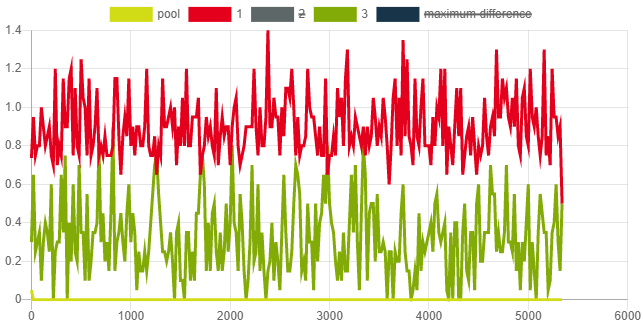
\includegraphics[width=0.8\textwidth]{media/simulation-divergence-chunks.PNG}
\end{figure}

In general, it can be seen that the ratio of chunks to participants may play a significant role in balancing the ease of achieving equilibrium. Despite the possibilities of significant losses, it is also possible to achieve a fairly distributed game if there exists the opportunity for participants to maintain possession of chunks across rounds.

\section{Demonstration} \label{section:demonstration}

A live example demonstrating a simple interactive game with a pool and two participants can be found live on \url{https://harberger-tax.netlify.app/} (as of Nov 1 2020) or in source code on Gitlab \footnote{\url{https://gitlab.com/harberger-tax/demonstration}}. As seen in \cref{figure:demonstration-start} below, the initial funds, chunks, and participation chance can be customised for each participant.

\begin{figure}[H]
  \centering
  \caption{Demonstration initialisation screen}
  \label{figure:demonstration-start}
  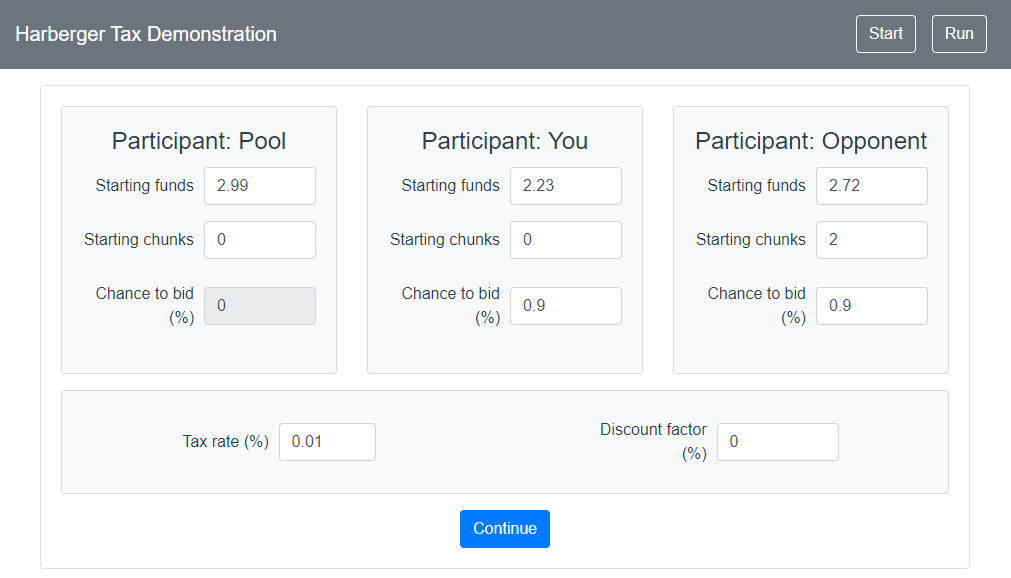
\includegraphics[width=\textwidth]{media/demonstration-start.PNG}
\end{figure}

As seen in \cref{figure:demonstration-run} below, the user is then able to initiate an auction (balance permitting), skip, the round, or let the action be determined randomly during their turn. During the opponents turn, the user may chose to particpate and make a bid or skip. The deterministic state generator has also been integrated to give the user a limited prediction of the game's possible outcomes in the near future.

\begin{figure}[H]
  \centering
  \caption{Demonstration run screen}
  \label{figure:demonstration-run}
  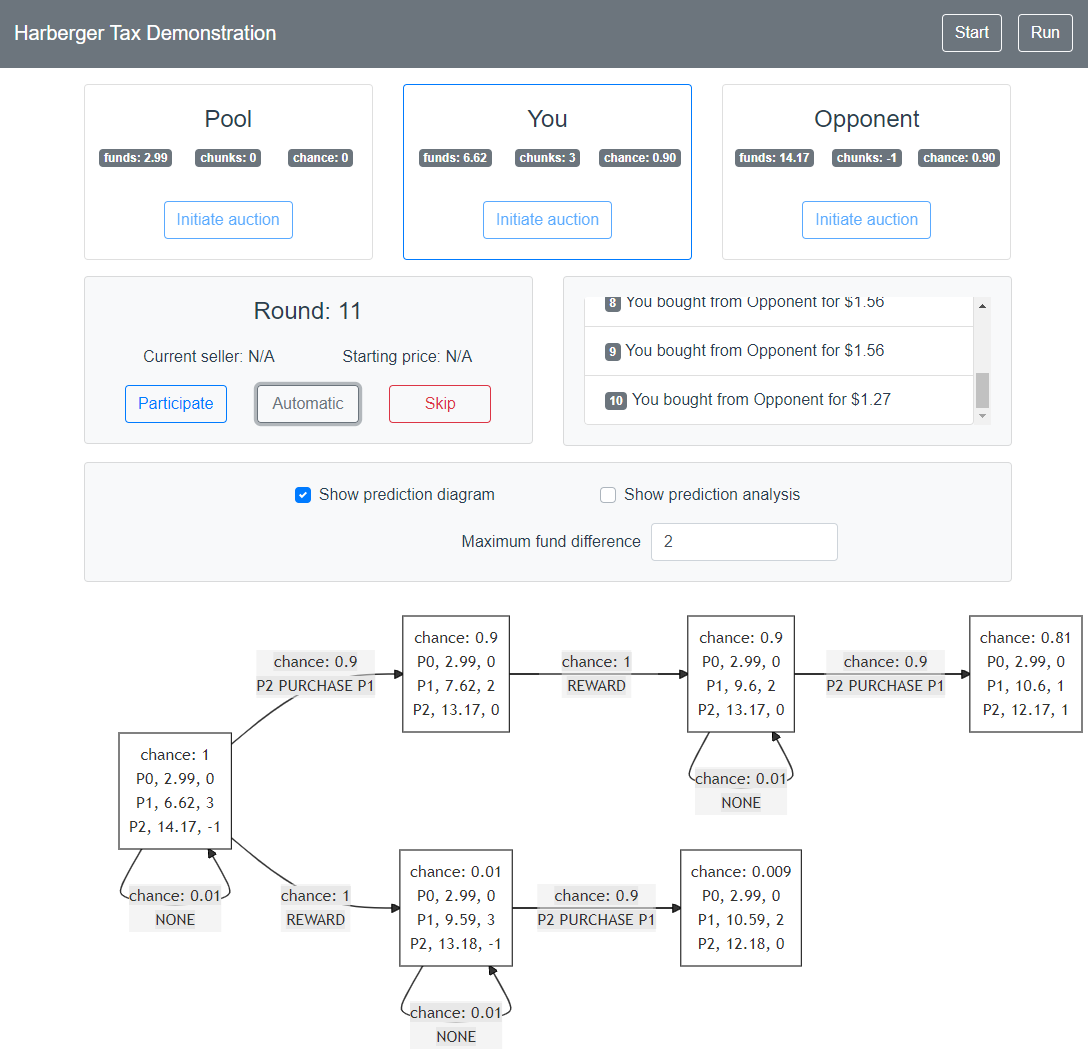
\includegraphics[width=\textwidth]{media/demonstration-run.PNG}
\end{figure}


%CONCLUSION CHAPTER
\chapter{Conclusion and Future Work}

% \todo[inline]{
%     emphasise that you've met your research aims \\
%     summarise the main findings of your research \\
%     restate the limitations of your research and make suggestions for further research.
% }

The Harberger Tax provides a viable economy as a starting point in ideal conditions. The probability of achieving the equilibrium state and maximising expected reward is heavily dependent on the willingness of a participant to actively engage in trading. However there exist limitations in terms of scalability and longevity as maintaining fairness requires balancing parameters such as taxation, trade interval versus block time, and the number of chunks per participant. Additionally, The stability and distributed nature is heavily reliant on implementation-specific mechanisms and the effects of integrating with a system that allocates computational power is still unknown.

While the results and analysis could have been more in-depth, there were some roadblocks encountered due to both hardware and experimental design limitations. Hence, there are several avenues of further investigation:

\begin{itemize}
    \item Extend state diagram generator to reach final states given hardware limitations (perhaps through a database or different language).
    \item Increasing complexity of simulation by allowing participants to join mid-game, allowing multi-chunk purchases, or by implementing different auction formats.
    \item Improve modelling of participants decision-making process.
    \item Explore mechanisms to facilitate a real-world implementation with a decentralised orchestrator (as a smart contract) or as a centralised authority.
    \item Using real-world values to evaluate the true profit or loss any participating entity may experience.
\end{itemize}



% ***************************************************
% Bibliography
%****************************************************
%CHOOSE YOUR BIB STYLE AND FILE.
%We have included the following two referencing styles for you to use in your thesis. You can add an alternate style if you prefer.

%Style: apalike = this is an (Author, Year) referencing style similar to APA
%Style: elsarticle-num = this is a numbered referencing style that will display the bibliography in citation order

%To use one of the styles provided ensure the % is removed from the start of the line, and the other option is commented out with a % at the start of the line. The style elsarticle-num is active by default.

%\bibliographystyle{apalike}
% \bibliographystyle{elsarticle-num}

% \bibliography{other/sources}

\printbibliography

%When you have finished your thesis we recommend that you manually fix any errors in your bibliography. 
%To do this, compile, copy the .bbl into a new .tex file and include this here after commenting out the other bibliography commands. Make corrections in that .tex file.

% ***************************************************
% Appendices
%**************************************************** 
%UNCOMMENT THIS SECTION IF YOU ARE USING APPENDICES.
%Simply adapt the same formatting used for other chapters.
\appendix
% If you need appendix in your thesis then consider the following appendix file (you can add more if you need more) otherwise you should not consider it in your main thesis.
\appendix

\begin{filecontents*}{media/state-generator-test-participation-probability.sh}
#!/bin/bash

X=(0.1 0.3 0.5 0.7 0.9)

for c1 in ${X[@]}; do
  for c2 in ${X[@]}; do
    node --max-old-space-size=10000 dist/index.js \
      --format csv \
      --output results/output-chance-$c1-$c2 \
      --tax 0 \
      --discount-factor 0 \
      --wealth-difference 5 \
      --max-depth 15 \
      --p1 $c1 --p2 $c2 | tee -a log
  done
done
\end{filecontents*}

\begin{filecontents*}{media/state-generator-test-participation-probability-taxed.sh}
#!/bin/bash

X=(0.1 0.3 0.5 0.7 0.9)

for c1 in ${X[@]}; do
  for c2 in ${X[@]}; do
    node --max-old-space-size=10000 dist/index.js \
      --format csv \
      --output results/output-chance-$c1-$c2 \
      --tax 0.2 \
      --discount-factor 0 \
      --wealth-difference 5 \
      --max-depth 15 \
      --p1 $c1 --p2 $c2 | tee -a log
  done
done
\end{filecontents*}

\begin{filecontents*}{media/state-generator-test-participation-tax.sh}
#!/bin/bash

X=(0 0.1 0.3 0.5 0.7 0.9)

for tax in ${X[@]}; do
  node --max-old-space-size=10000 dist/index.js \
    --format csv \
    --output results/output-tax-$tax \
    --tax $tax \
    --discount-factor 0 \
    --wealth-difference 5 \
    --max-depth 15 \
    --p1 0.9 --p2 0.9 | tee -a log
done;

\end{filecontents*}

\begin{filecontents*}{media/hashrate-distribution.csv}
Pool,Blocks Mined
Unknown,26
F2Pool,20
Poolin,12
AntPool,10
Huobi.pool,9
ViaBTC,6
1THash\&58COIN,6
NovaBlock,3
BTC.com,2
BTC.TOP,1
SlushPool,1
\end{filecontents*}

\begin{filecontents*}{media/state-results.csv}
p1,p2,Expected,Expected (taxed),Best,Best (taxed),Worst,Worst (taxed)
0.1,0.1,1.88,2.37,4.30E-06,5.31E-06,3.49E-05,3.14E-04
0.1,0.3,0.80,1.60,4.25E-05,6.75E-05,1.15E-04,1.03E-03
0.1,0.5,0.21,0.77,5.13E-05,1.14E-04,8.30E-05,7.47E-04
0.1,0.7,0.05,0.24,1.82E-05,6.75E-05,2.11E-05,1.90E-04
0.1,0.9,0.03,0.07,4.78E-07,5.31E-06,4.30E-07,3.87E-06
0.3,0.1,1.36,2.72,1.42E-05,2.25E-05,6.95E-05,1.62E-04
0.3,0.3,0.62,2.24,1.40E-04,2.86E-04,2.29E-04,5.34E-04
0.3,0.5,0.25,1.47,1.69E-04,4.82E-04,1.65E-04,3.86E-04
0.3,0.7,0.33,1.25,6.00E-05,2.86E-04,4.20E-05,9.81E-05
0.3,0.9,0.74,1.68,1.58E-06,2.25E-05,8.58E-07,2.00E-06
0.5,0.1,0.47,1.48,1.03E-05,2.28E-05,2.56E-05,2.56E-05
0.5,0.3,0.33,1.72,1.01E-04,2.89E-04,8.44E-05,8.44E-05
0.5,0.5,0.55,2.44,1.22E-04,4.88E-04,6.10E-05,6.10E-05
0.5,0.7,1.54,4.99,4.34E-05,2.89E-04,1.55E-05,1.55E-05
0.5,0.9,4.51,10.64,1.14E-06,2.28E-05,3.16E-07,3.16E-07
0.7,0.1,0.08,0.43,2.60E-06,9.64E-06,2.34E-06,1.00E-06
0.7,0.3,0.40,1.48,2.57E-05,1.23E-04,7.72E-06,3.31E-06
0.7,0.5,1.61,5.19,3.10E-05,2.07E-04,5.58E-06,2.39E-06
0.7,0.7,5.69,15.63,1.10E-05,1.23E-04,1.42E-06,6.08E-07
0.7,0.9,18.02,41.01,2.89E-07,9.64E-06,2.89E-08,1.24E-08
0.9,0.1,0.03,0.10,5.31E-08,5.90E-07,5.31E-09,5.90E-10
0.9,0.3,0.81,1.94,5.25E-07,7.50E-06,1.75E-08,1.94E-09
0.9,0.5,4.65,11.15,6.33E-07,1.27E-05,1.27E-08,1.41E-09
0.9,0.7,18.09,41.45,2.25E-07,7.50E-06,3.21E-09,3.57E-10
0.9,0.9,54.53,119.69,5.90E-09,5.90E-07,6.56E-11,7.29E-12
\end{filecontents*}

\begin{filecontents*}{media/state-results-tax.csv}
Tax,Expected
0,54.53
0.1,43.71
0.3,33.99
0.5,24.28
0.7,12.14
0.9,0.65
\end{filecontents*}

\begin{filecontents*}{media/model.prism}
csg

player p0 P0 endplayer
player p1 P1 endplayer
player p2 P2 endplayer

const int MAX_STEPS = 999;
const int MAX_INT = 99;

const int STAGE_NONE = -1;
const int STAGE_DECIDE = 0;
const int STAGE_PURCHASE = 1;

const int NOPLAYER = -1;
const int PLAYER0 = 0;
const int PLAYER1 = 1;
const int PLAYER2 = 2;

const double p;
const double q;
const double tr;
const double dr;

formula discounted_tax = 1 / pow(1 + tr, steps / 2);

formula current_tax = discounted_tax > dr ? discounted_tax : 0;

formula current_stage = steps < MAX_STEPS 
  ? mod(steps, 2) 
  : STAGE_NONE;

module P0

  c0 : [0..MAX_INT] init 2;

  [decide_0] current_stage = STAGE_DECIDE -> true;

  [transact_0] current_stage = STAGE_PURCHASE & c0 > 0 ->
    (
      c0' = d1 = PLAYER0 & d2 = PLAYER0 
        ? c0 - 2 
        : d1 = PLAYER0 | d2 = PLAYER0
        ? c0 - 1
        : c0
    );

endmodule

module P1

  c1 : [0..MAX_INT] init 0;
  d1 : [-1..2] init NOPLAYER;

  [decide_1] current_stage = STAGE_DECIDE ->
    p / 2 : (d1' = c2 > 0 ? PLAYER2 : c0 > 0 ? PLAYER0 : NOPLAYER) +
    p / 2 : (d1' = c0 > 0 ? PLAYER0 : c2 > 0 ? PLAYER2 : NOPLAYER) +
    1 - p : true;

  [transact_1] current_stage = STAGE_PURCHASE ->
    (
      c1' = d2 = PLAYER1 & d1 = NOPLAYER
        ? c1 - 1
        : d2 != PLAYER1 & d1 != NOPLAYER
        ? c1 + 1
        : c1
    );

endmodule

module P2

  c2 : [0..MAX_INT] init 0;
  d2 : [-1..2] init NOPLAYER;

  [decide_2] current_stage = STAGE_DECIDE ->
    q / 2 : (d2' = c1 > 0 ? PLAYER1 : c0 > 0 ? PLAYER0 : NOPLAYER) +
    q / 2 : (d2' = c0 > 0 ? PLAYER0 : c1 > 0 ? PLAYER1 : NOPLAYER) +
    1 - q : true;

  [transact_2] current_stage = STAGE_PURCHASE ->
    (
      c2' = d1 = PLAYER2 & d2 = NOPLAYER
        ? c2 - 1
        : d1 != PLAYER2 & d2 != NOPLAYER
        ? c2 + 1
        : c2
    );

endmodule

module Game

  steps : [0..MAX_STEPS] init 0;

  [] steps < MAX_STEPS & current_tax > 0 -> (steps' = steps + 1);

endmodule

rewards "p0"

  [decide_0] true : c0 * current_tax;

  [transact_0] true : d1 = PLAYER0 & d2 = PLAYER0 
    ? 2 
    : d1 = PLAYER0 | d2 = PLAYER0
    ? 1
    : 0;

endrewards

rewards "p1"

  [decide_1] true : c1 * current_tax;
  
  [transact_1] true : d2 = PLAYER1 & d1 = NOPLAYER
    ? 1
    : d2 != PLAYER1 & d1 != NOPLAYER
    ? -1
    : 0;

endrewards

rewards "p2"

  [decide_2] true : c2 * current_tax;

  [transact_2] true : d1 = PLAYER2 & d2 = NOPLAYER
    ? 1
    : d1 != PLAYER2 & d2 != NOPLAYER
    ? -1
    : 0;

endrewards

\end{filecontents*}

\chapter{Test Scripts}

\section{Deterministic State Generator}

\subsection{Participation Probability} \label{appendix:testparticipationprobability}

\verbatiminput{media/state-generator-test-participation-probability.sh}

\subsection{Participation Probability Taxed} \label{appendix:testparticipationprobabilitytaxed}

\verbatiminput{media/state-generator-test-participation-probability-taxed.sh}

\subsection{Taxation Rate} \label{appendix:testparticipationtax}

\verbatiminput{media/state-generator-test-participation-tax.sh}

\chapter{Raw Data}

\section{Experimentation System Details} \label{appendix:computerspecs}

The computer on which all experiments were executed has the following specifications:

\begin{itemize}
    \item CPU - AMD Ryzen 5 2600, 6 Cores, 12 Threads at 3.4GHz
    \item RAM - 16GB DDR4
\end{itemize}

\section{Hash-rate Distribution} \label{appendix:hashrate-distribution}

Data retrieved from \cite{bitcoinhashrate2020}.
\begin{table}[H]
    \centering
    \csvautotabular{media/hashrate-distribution.csv}
    \caption{Distribution of mined blocks per pool over a 24 hour period}
    \label{table:hashrate-distribution}
\end{table}

\section{Deterministic State Generator Variable Participation Chance Results} \label{appendix:state-results}

\begin{table}[H]
    \centering
    \csvautotabular{media/state-results.csv}
    \caption{Metrics retrieved from test script (\cref{appendix:testparticipationprobability})}
    \label{table:testparticipationprobability}
\end{table}


\section{Deterministic State Generator Variable Participation Chance Results} \label{appendix:state-results-tax}

\begin{table}[H]
    \centering
    \csvautotabular{media/state-results-tax.csv}
    \caption{Metrics retrieved from test script (\cref{appendix:testparticipationtax})}
    \label{table:testparticipationprobability}
\end{table}

\chapter{Code}

\section{PRISM-games CSG Model}
\label{appendix:prism-model}

\verbatiminput{media/model.prism}

% ***************************************************
% Examples
%**************************************************** 
% The following files are only for examples and you should not include them in your final thesis.
% % ***************************************************
% Example of Citations
% ***************************************************
%This example is provided for your reference only. DO NOT INCLUDE IN YOUR FINAL THESIS. 
\chapter{Example of Citations}

This text is only for Bibliography testing purposes. This is a book by Cawvey et al.~\cite{Cawvey2017}. There are few journal articles~\cite{Pakzad2018, Adachi2007} in this bibliography. This is a proceeding paper~\cite{J.Fenwick2010}.  This is a PhD thesis by Peerling~\cite{PeerlingPhD1999}. These are few other types of citations~\cite{Panis2004}.
% % ***************************************************
% Example of Code; how to import Code in pdf.
% ***************************************************
%This example is provided for your reference only. DO NOT INCLUDE IN YOUR FINAL THESIS. 
\chapter{Example of Code}

\section{Find the greatest number from a list of numbers in \textit{Python}}

\begin{verbatim}

a=[1,2,3,4,6,7,99,88,999]
    max= 0
    for i in a:
        if i > max:
            max=i
    print(max)

\end{verbatim}
% % ***************************************************
% Example of Equations
% ***************************************************
%This example is provided for your reference only. DO NOT INCLUDE IN YOUR FINAL THESIS. 
\chapter{Example of Equations}

\begin{equation}
    E = mc^2
\end{equation}


\begin{align}
    a = {}& b + c\\
    x = {}& y + z
\end{align}


\begin{equation}
    \begin{split}
        a = {}& b + c\\
            {}& + d + e
    \end{split} 
\nonumber
\end{equation}
    
    
\begin{equation} 
sinx+cosx=1 
\end{equation}



% % ***************************************************
% Example of Figures
% ***************************************************
%This example is provided for your reference only. DO NOT INCLUDE IN YOUR FINAL THESIS. 

%\begin{figure} : If you put no command after \begin{table} then this figure will be printed anywhere in your pdf where LaTex finds the free space to put it. If you wish to specify where the figure goes you have to give a command in LaTex after  \begin{figure}. 
%
%There are different commands to put the figure in different positions e.g. \begin{table}[h] LaTex will print the figure in the same position that you put it in your source file, if there is enough space to print it
%N.B. it is important to note that commanding LaTeX to add a figure in a specific place may result in formatting issues.

\chapter{Example of Figures}

\begin{figure}[h]
\begin{center}
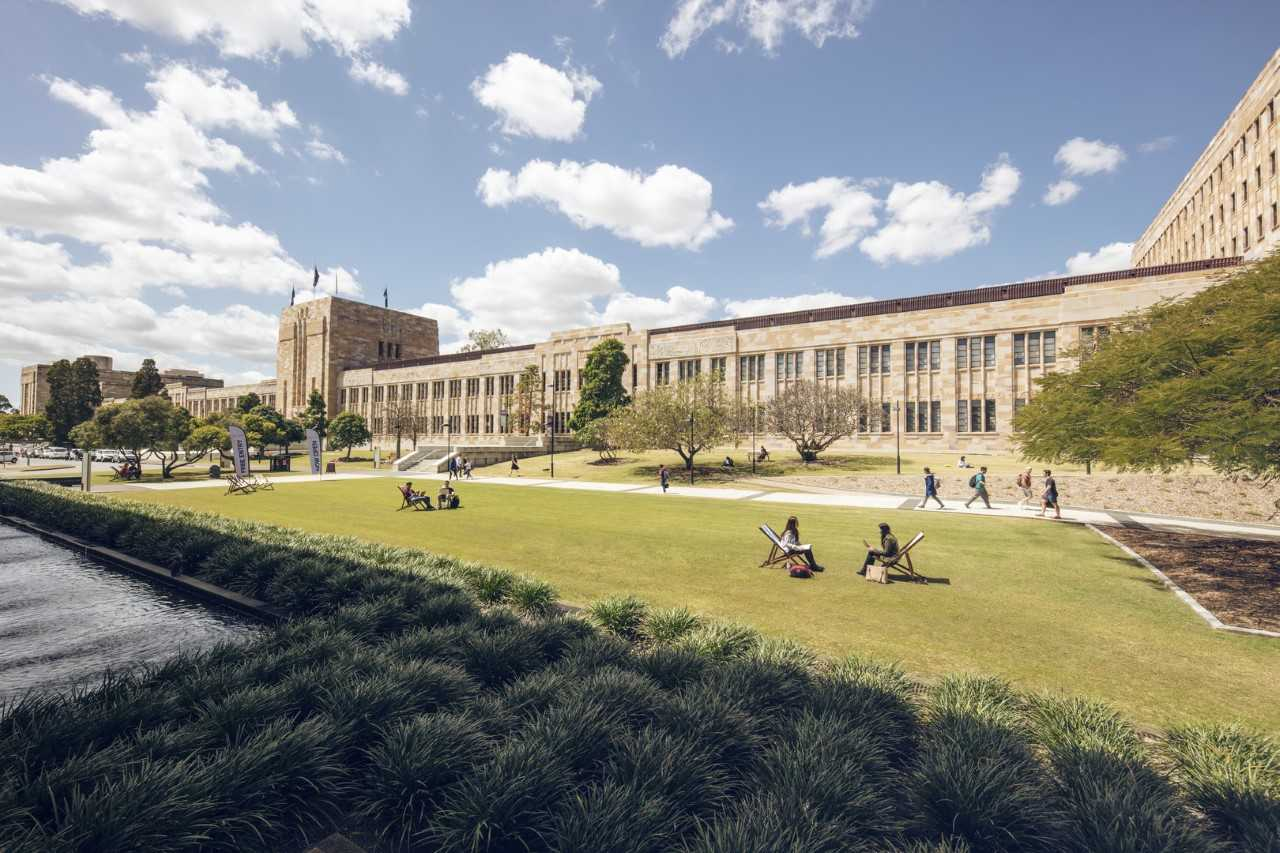
\includegraphics[width=1.0\textwidth]{Examples/FigureUQ}
\caption{The University Of Queensland}
\label{Fig:1}
\end{center}
\end{figure}

The Figure~\ref{Fig:1} represents beauty of the UQ campus.
% % ***************************************************
% Example of Flow Charts
% ***************************************************
%This example is provided for your reference only. DO NOT INCLUDE IN YOUR FINAL THESIS. 
\chapter{Example of Flow Charts}
\begin{figure}[h]
\caption{Flow Chart}
\label{Fig:FlowChart}
\begin{center}
\tikzstyle{decision} = [diamond, draw, fill=white!10, 
    text width=4.5em, text badly centered, node distance=3cm, inner sep=0pt]
\tikzstyle{block} = [rectangle, draw, fill=white!20, 
    text width=5em, text centered, rounded corners, minimum height=4em]
\tikzstyle{line} = [draw, -latex']
\tikzstyle{cloud} = [draw, ellipse,fill=white!20, node distance=3cm,
    minimum height=2em]
    
\begin{tikzpicture}[node distance = 2cm, auto]
    % Place nodes
    \node [block] (Step1) {initialize model};
    \node [cloud, left of=Step1] (expert) {expert};
    \node [cloud, right of=Step1] (system) {system};
    \node [block, below of=Step1] (identify) {identify candidate models};
    \node [block, below of=identify] (evaluate) {evaluate candidate models};
    \node [block, left of=evaluate, node distance=3cm] (update) {update model};
    \node [decision, below of=evaluate] (decide) {is best candidate better?};
    \node [block, below of=decide, node distance=3cm] (stop) {stop};
    % Draw edges
    \path [line] (Step1) -- (identify);
    \path [line] (identify) -- (evaluate);
    \path [line] (evaluate) -- (decide);
    \path [line] (decide) -| node [near start] {yes} (update);
    \path [line] (update) |- (identify);
    \path [line] (decide) -- node {no}(stop);
    \path [line,dashed] (expert) -- (Step1);
    \path [line,dashed] (system) -- (Step1);
    \path [line,dashed] (system) |- (evaluate);
\end{tikzpicture}
\end{center}
\end{figure}

Flow chart~\ref{Fig:FlowChart} is a simple example.
% % ***************************************************
% Example of Tables
% ***************************************************
%This example is provided for your reference only. DO NOT INCLUDE IN YOUR FINAL THESIS. 
\chapter{Example of Tables}

Here is a really simple table~\ref{Table}.


%\begin{table} : If you put no command after \begin{table} then this table will be printed anywhere in your pdf where LaTex finds the free space to put it. If you wish to specify where the table goes you have to give a command in LaTex after  \begin{table}. 
%
%There are different commands to put the table in different positions e.g. \begin{table}[h] LaTex will print the table in the same position that you put it in your source file, if there is enough space to print it
%N.B. it is important to note that commanding LaTeX to add a table in a specific place may result in formatting issues.

\begin{table}[h]
\caption{Name of the Australian Cities}
\begin{center}
\begin{tabular}{{|c|c|c|}}
\hline
\textbf{Number}& \textbf {Name}\\
\hline
      1& Brisbane\\
      2& Sydney\\
      3& Melbourne\\
      4& Canberra\\
      5& Perth\\
      6& Adelaide\\
      7& Hobart\\
      8& Darwin\\
\hline
\end{tabular}
\end{center}
\label{Table}
\end{table}


% ***************************************************
% Back Matter
%**************************************************** 
%COMMENT OUT IF YOU DO NOT WISH TO INCLUDE BACK MATTER.
% % ***************************************************
% Back Matter
% ***************************************************
% ADD AN ENDQUOTE HERE. If you do not wish to, delete this file.
\backmatter

\normalfont
\cleartooddpage

\pagestyle{empty}

\begin{table}[b!]
\begin{center}
% ********* Enter your quote within {} brackets: ********
\textit{Endquote goes here.}

% ********************************************************
\end{center}
\begin{flushright}
% ********* Enter your text below, as indicated: ********
Author of quote,\\
Source of quote

% ********************************************************
\end{flushright}
\end{table}

\end{document}
